
\section{Robustness checks and implementation details for the simulations in Section \ref{sec-sim}}\label{sec-supp-sim}


\subsection*{Implementation of SiZer in Section \ref{subsec-sim-multiscale}}


\textcolor{red}{The SiZer methods in Section \ref{subsec-sim-multiscale} are implemented as follows:}
\begin{enumerate}[leftmargin=0.7cm,label=(\alph*)]

\item Computation of the grid $\mathcal{G}_T^*$:

To start with, we compute the variance of $\bar{Y} = T^{-1} \sum_{t=1}^T Y_{t,T}$, which is given by
\[ \var(\bar{Y}) = \frac{\gamma_\varepsilon(0)}{T} + \frac{2}{T} \sum_{k = 1}^{T-1} \Big(1 - \frac{k}{T}\Big)\gamma_\varepsilon(k). \]
Since the autocovariance function $\gamma_{\varepsilon}(\cdot)$ is known by assumption, we can calculate the value of $\var(\bar{Y})$ by using the formula $\gamma_\varepsilon(k) = \nu^2 a_1^{|k|} / (1 - a_1^2)$ together with the true para\-meters $a_1$ and $\nu^2 = \ex[\eta_t^2]$. We next compute 
\[ T^* = \frac{\gamma_\varepsilon(0)}{\var(\bar{Y})}, \]
which can be interpreted as a measure of information in the data. \textcolor{red}{For each point $(u,h) \in \mathcal{G}_T$}, we finally calculate the effective sample size for dependent data 
\[ \text{ESS}^*(u, h) = \frac{T^*}{T} \frac{\sum_{t=1}^T K_h(t/T - u)}{K_h(0)} \]
with $K_h(v) = h^{-1} K(v/h)$ and set $\mathcal{G}_T^* = \{ (u,h) \in \mathcal{G}_T: \text{ESS}^*(u, h) \ge 5 \}$. 

\item Computation of the local linear estimators and their standard deviations: 

For each $(u,h) \in \mathcal{G}_T^*$, we compute a standard local linear estimator $\widehat{m}^\prime_h(u)$ of the derivative $m^\prime(u)$ together with its standard deviation $\text{sd}(\widehat{m}^\prime_h(u))$. The latter is given by $\text{sd}(\widehat{m}^\prime_h(u)) = \{ \var(\widehat{m}^\prime_h(u)) \}^{1/2}$, where $\var(\widehat{m}^\prime_h(u)) = e^\top V e$ with $e = (\begin{matrix} 0 & 1 \end{matrix})^\top$ and 
\[ V = (X^T W X)^{-1} (X^T \Sigma X) (X^T W X)^{-1}. \]
The matrices $X$, $W$ and $\Sigma$ are defined as follows: $\Sigma$ is a $T \times T$ matrix with the elements
\[ \Sigma_{st} = \gamma_\varepsilon(s-t) K_h\Big( \frac{s}{T} - u \Big) K_h\Big( \frac{t}{T} - u \Big), \]
$W$ is a $T \times T$ diagonal matrix with the diagonal entries $K_h(t/T-u)$ and 
\[ X =   
\begin{pmatrix}
1 & (1/T - u)   \\
1 & (2/T - u)   \\
\vdots & \vdots \\
1 & (1 - u)     \\
\end{pmatrix}. \]

\item Computation of the confidence intervals:  

For a given confidence level $\alpha$ and for each bandwidth value $h$ with $(u,h) \in \mathcal{G}_T^*$, we compute the quantile 
\[ q(h) = \Phi^{-1} \Big( \Big( 1 - \frac{\alpha}{2} \Big)^{1/(\theta g)} \Big), \]
where $\Phi$ is the distribution function of a standard normal random variable, $g$ is the number of locations $u$ in the grid $\mathcal{G}_T$, and the cluster index $\theta$ is defined on p.1519 in \cite{ParkHannigKang2009}. The confidence interval of $\widehat{m}^\prime_h(u)$ is then computed as $[\widehat{m}^\prime_h(u) - q(h) \, \text{sd}(\widehat{m}^\prime_h(u)),\widehat{m}^\prime_h(u) + q(h) \, \text{sd}(\widehat{m}^\prime_h(u))]$. 

%For each $(u,h) \in \mathcal{G}_T^*$, we compute the Gaussian quantile for the confidence level $\alpha$
%\[ q(u,h) = \Phi^{-1} \Big(\frac{1 + (1 - \alpha)^{\frac{1}{l(u, h)}}}{2}\Big), \]
%where $l(u,h) = T/\text{ESS}^*(u, h)$ and $\Phi$ is the distribution function of a standard normal random variable. The confidence interval of $\widehat{m}^\prime_h(u)$ is then computed as $[\widehat{m}^\prime_h(u) - q(u,h) \, \text{sd}(\widehat{m}^\prime_h(u)),\widehat{m}^\prime_h(u) + q(u,h) \, \text{sd}(\widehat{m}^\prime_h(u))]$. 

\end{enumerate}


\subsection*{Power simulations additional to Section \ref{subsec-sim-multiscale-power}}


In the following simulation exercises, we compare the performance of the tests $\mathcal{T}_{\text{MS}}$, $\mathcal{T}_{\text{UC}}$, $\mathcal{T}_{\text{RW}}$ and $\mathcal{T}_{\text{SiZer}}$ (i) when $m$ is the blocks signal of \cite{DonohoJohnstone1995} that was investigated in detail by \cite{HannigMarron2006} in the SiZer context and (ii) when $m$ is the sine curve $m(u) = \sin(6\pi u)$ that was considered in \cite{ParkHannigKang2009}. We define the blocks signal exactly as \cite{MarronAdakJohnstoneNeumannPatil1998} and \cite{HannigMarron2006}. Specifically, we set 
\begin{align*}
m(x) = (0.6/9.2) 
 & \big\{ 4 \text{ssgn}(x-0.1) - 5 \text{ssgn}(x-0.13) + 3 \text{ssgn}(x-0.15) \\ 
 & - 4 \text{ssgn}(x-0.23) + 5 \text{ssgn}(x-0.25) -4.2 \text{ssgn}(x-0.4) \\
 & + 2.1 \text{ssgn}(x-0.44) + 4.3 \text{ssgn} (x-0.65) - 3.1\text{ssgn}(x-0.76) \\
 & + 2.1 \text{ssgn}(x-0.78) - 4.2 \text{ssgn}(x-0.81) + 2 \big\} + 0.2,
\end{align*}
where $\text{ssgn}(x) = (1+\text{sgn}(x))/2$ is a shifted version of the standard sign function $\text{sgn}(x)$. In both the blocks and the sine case, we model the error terms as an AR($1$) process $\varepsilon_t = a_1 \varepsilon_{t-1} + \eta_1$, where $a_1 \in\{-0.5,0.5\}$ and $\eta_t$ are i.i.d.\ normal with $\ex[\eta_t] = 0$ and $\ex[\eta_t^2] = \nu^2$. In the blocks example, we set $\nu^2 = (1-a_1^2)/100$. This implies that $\var(\varepsilon_t) = (0.1)^2$, which matches the variance of the i.i.d.\ errors in the blocks example of \cite{HannigMarron2006}. In the sine example, we choose $\nu^2 = (1-a_1^2)$, which implies that $\var(\varepsilon_t) = 1$. A plot of the blocks signal is given in the two top panels of Figure \ref{fig:sizer:blocks}. As can be seen, the signal is a piecewise constant function with several jumps. We could replace this jump function by a slightly smoothed and thus differentiable version with very steep increases and decreases. However, as this would leave the simulation results essentially unchanged, we stick to the original blocks signal.  


For both the blocks and the sine example, we simulate a representative data sample of length $T=1000$ and carry out the four tests on the simulated sample for the significance level $\alpha=0.05$. The results are presented by SiZer maps in Figures \ref{fig:sizer:blocks} and \ref{fig:sizer:sine} which are to be read as follows: Each pixel of the SiZer map corresponds to a location-scale point $(u,h)$, or put differently, to a time interval $[u-h,u+h]$. The pixel ($u,h)$ is coloured blue if the test finds an increase in the trend $m$ on the interval $[u-h,u+h]$, red if the test finds a decrease and purple if the test does not reject the null hypothesis that $m$ is constant on $[u-h,u+h]$. Moreover, a pixel $(u,h)$ is coloured grey if the effective sample size $\text{ESS}^*(u,h)$ is smaller than $5$, in which case the pixel $(u,h)$ is not included in the location-scale grid $\mathcal{G}_T^*$.


The results for the blocks example are reported in Figure \ref{fig:sizer:blocks}, the left-hand panels of subfigure (a) corresponding to the case with $a_1=-0.5$ and the right-hand panels of subfigure (b) to the case with $a_1=0.5$. Let us first have a closer look at subfigure (a). The top panel depicts the blocks signal with the simulated data sample in the background. The other panels show the SiZer maps produced by the four tests $\mathcal{T}_{\text{MS}}$, $\mathcal{T}_{\text{UC}}$, $\mathcal{T}_{\text{RW}}$ and $\mathcal{T}_{\text{SiZer}}$. As can be seen, the SiZer maps are fairly similar. In particular, all four tests pick up the increases and decreases (that is, the upward and downward jumps) in the signal $m$ quite accurately. The situation is a bit different in subfigure (b), that is, in the case with $a_1=0.5$. Overall, the colour patterns in the four SiZer maps look fairly similar. However, on closer inspection, the following differences become apparent: 
\begin{enumerate}[leftmargin=0.8cm,label=(\roman*)]
%\item The blue and red regions are tenedetially larger for the SiZer plots of the row-wise methods. 

\item In the SiZer maps of the two row-wise methods $\mathcal{T}_{\text{RW}}$ and $\mathcal{T}_{\text{SiZer}}$, there is a small strip of blue pixels around the jump location $u=0.44$. Hence, the row-wise methods detect the small upward jump in the blocks signal at $u=0.44$, whereas the global methods do not pick up this jump. 

\item In the SiZer map of $\mathcal{T}_{\text{SiZer}}$, there are two small strips of red pixels near the location $u=0.95$ corresponding to scales $h$ with $\log_{10}(h)$ between $-1.2$ and $-1.6$. Hence, the row-wise SiZer test $\mathcal{T}_{\text{SiZer}}$ spuriously finds a decrease in the trend $m$ on a short time interval around $u=0.95$. As a specific example, the pixel $(u,h) = (0.93,0.03)$ is coloured red, implying that $\mathcal{T}_{\text{SiZer}}$ spuriously finds a decrease on the interval $[0.90,0.96]$. Inspecting the grey time series plot in the top panel of subfigure (b), it indeed looks as if there is a short downward trend in the time series towards the end of the sample. However, this downward movement of the time series is not due to an actual decrease in the trend function $m$. It is rather produced by the autocorrelation structure in the error terms. 

\end{enumerate}
(i) indicates that the row-wise methods  $\mathcal{T}_{\text{RW}}$ and $\mathcal{T}_{\text{SiZer}}$ tend to be more powerful than the global tests $\mathcal{T}_{\text{MS}}$ and $\mathcal{T}_{\text{UC}}$. (ii) shows that this gain of power comes at a cost: The row-wise methods tend to find spurious increases/decreases more often than the global ones. Hence, the SiZer maps of subfigure (b) nicely illustrate the main findings of our power simulations in Section \ref{subsec-sim-multiscale-power}.


The SiZer maps for the sine example are depicted in Figure \ref{fig:sizer:sine}. Overall, they convey a picture very similar to the SiZer maps of the blocks example. The SiZer maps for the case with $a_1=-0.5$ show that the increases and decreases of the sine curve $m$ are picked up appropriately by all four tests. In the case with $a_1=0.5$, in contrast, the four tests only detect the increases and decreases of $m$ in the interior of the support $[0,1]$. The increase of $m$ at the left-hand boundary of the support is not picked up by any of the tests, the increase at the right-hand boundary is only detected by row-wise SiZer $\mathcal{T}_{\text{SiZer}}$, which is indicated by the small blue area at the right-hand boundary of the SiZer map. This again illustrates that the row-wise methods tend to be more powerful than the global tests. 


\begin{figure}[p]
\begin{subfigure}[b]{0.475\textwidth}
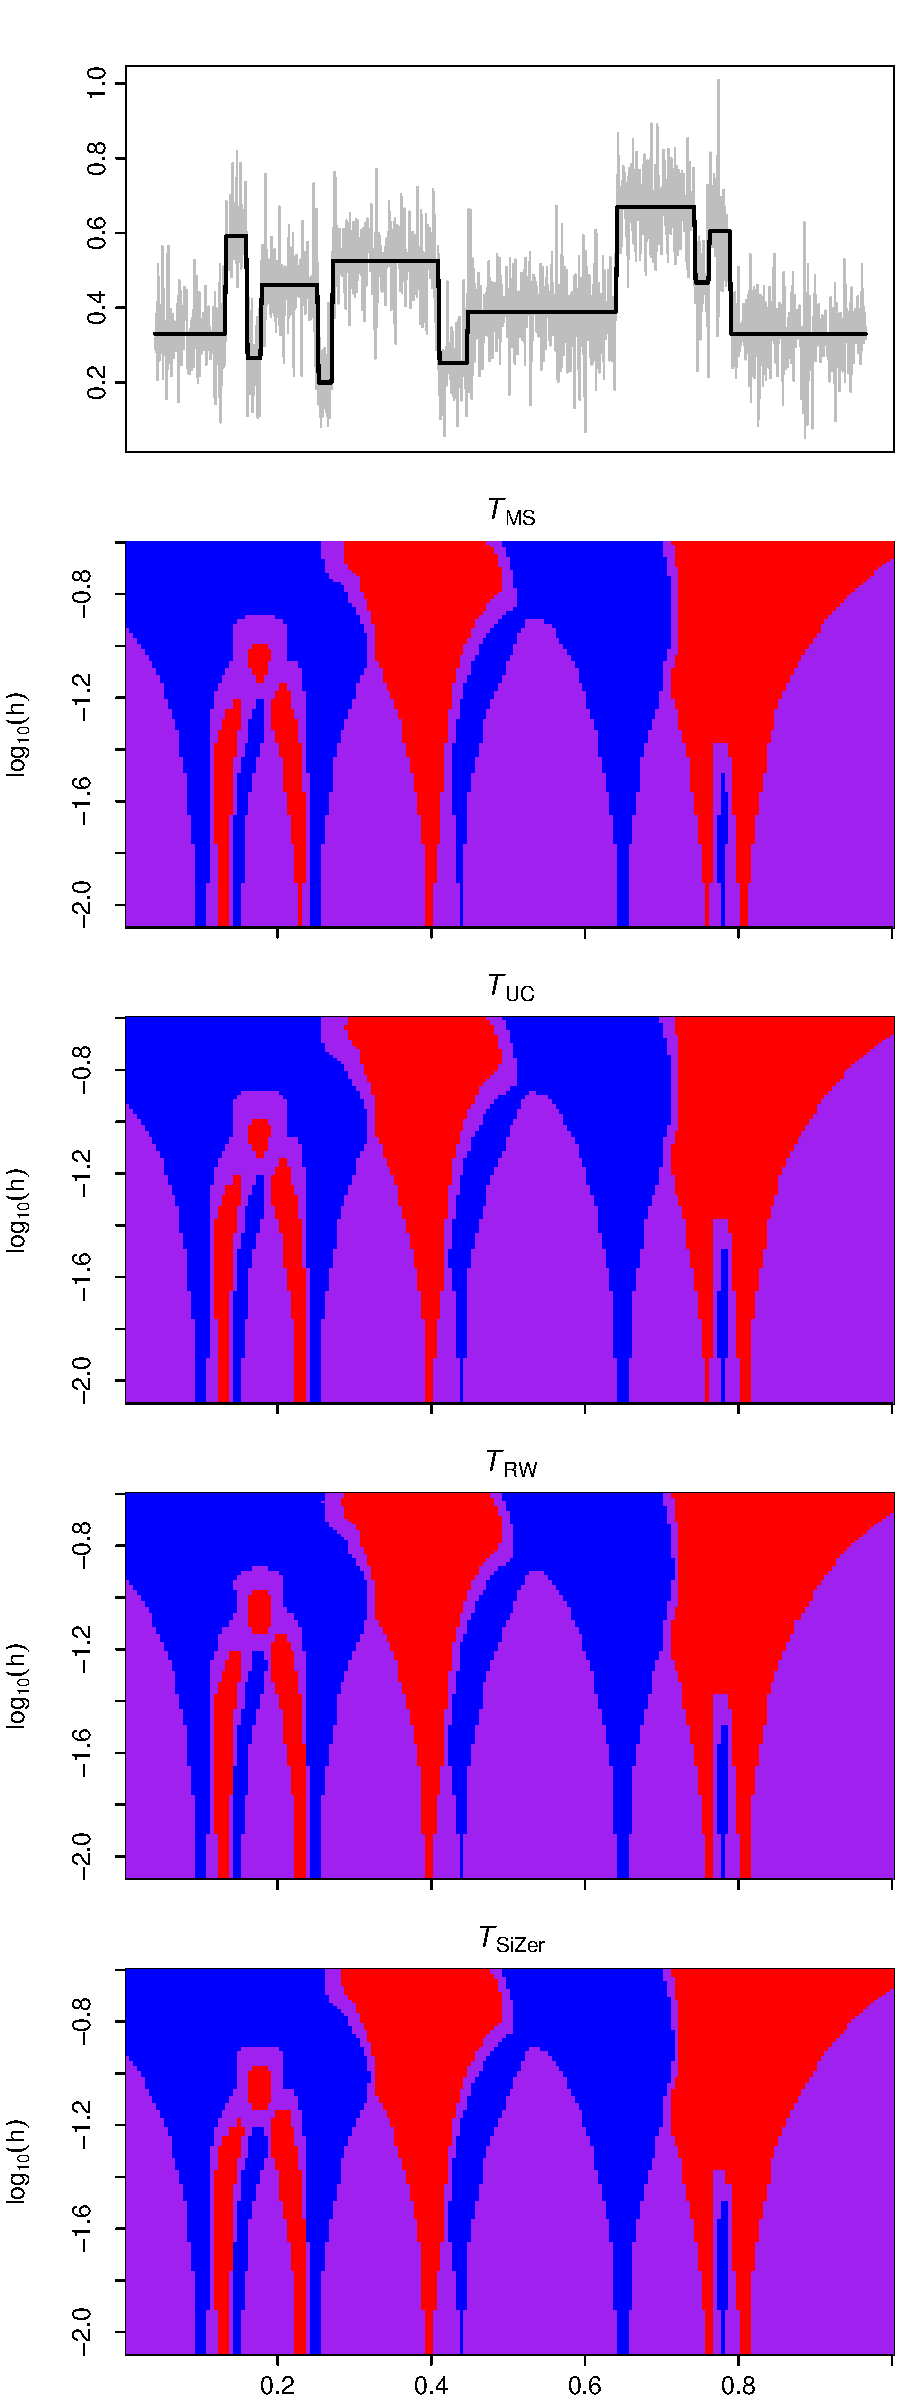
\includegraphics[width=\textwidth]{Plots/SiZermaps/SiZer_map_T_1000_blocks_a1_-50_seed_1.pdf}
\caption{$a=-0.5$}
\end{subfigure}
\hspace{0.25cm}
\begin{subfigure}[b]{0.475\textwidth}
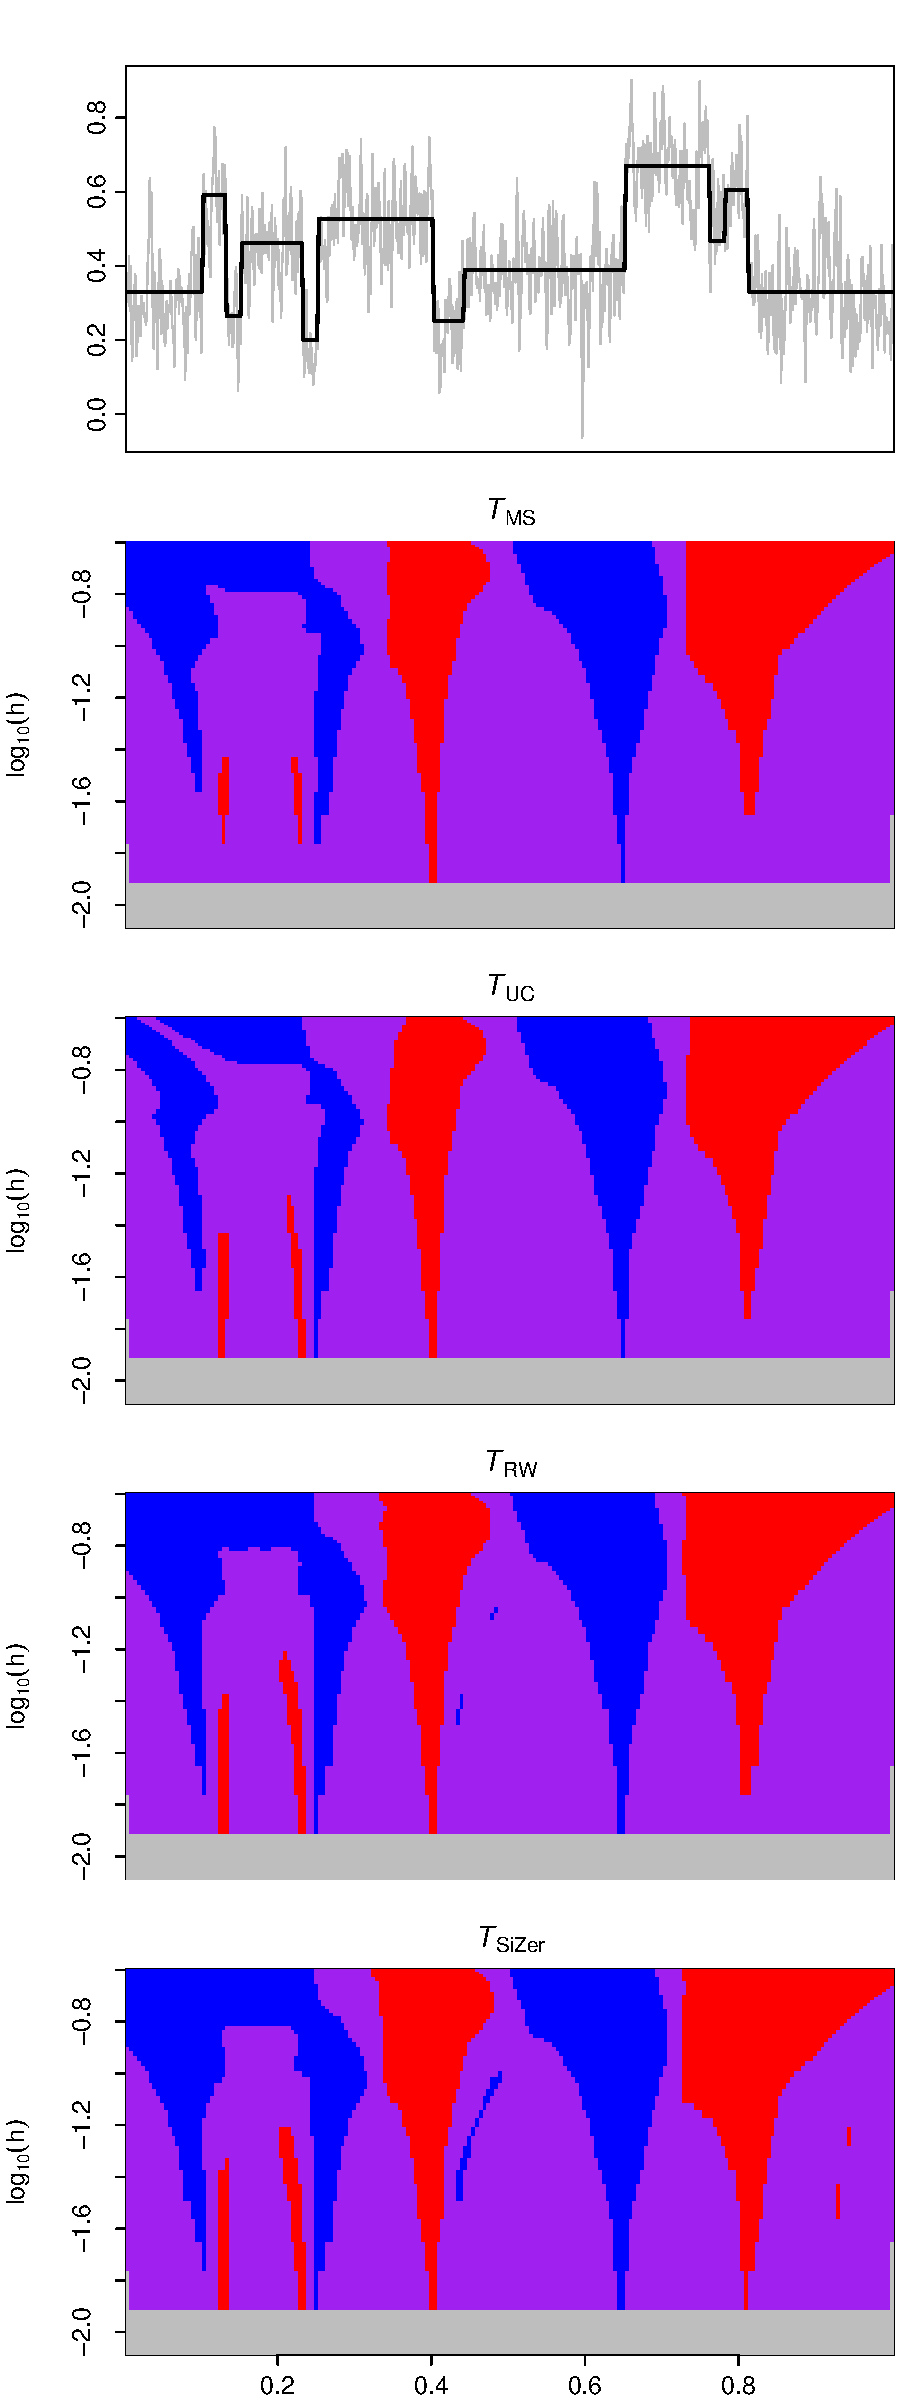
\includegraphics[width=\textwidth]{Plots/SiZermaps/SiZer_map_T_1000_blocks_a1_50_seed_6.pdf}
\caption{$a=0.5$}
\end{subfigure}
\caption{SiZer maps for the blocks example. The left-hand panels of subfigure (a) show the results for $a_1=-0.5$, the right-hand panels of subfigure (b) those for $a_1=0.5$. The two upper panels depicts the sine curve with the simulated data sample in the background. The other panels show the SiZer maps produced by the four tests $\mathcal{T}_{\text{MS}}$, $\mathcal{T}_{\text{UC}}$, $\mathcal{T}_{\text{RW}}$ and $\mathcal{T}_{\text{SiZer}}$.}\label{fig:sizer:blocks}
\end{figure}


\begin{figure}[p]
\begin{subfigure}[b]{0.475\textwidth}
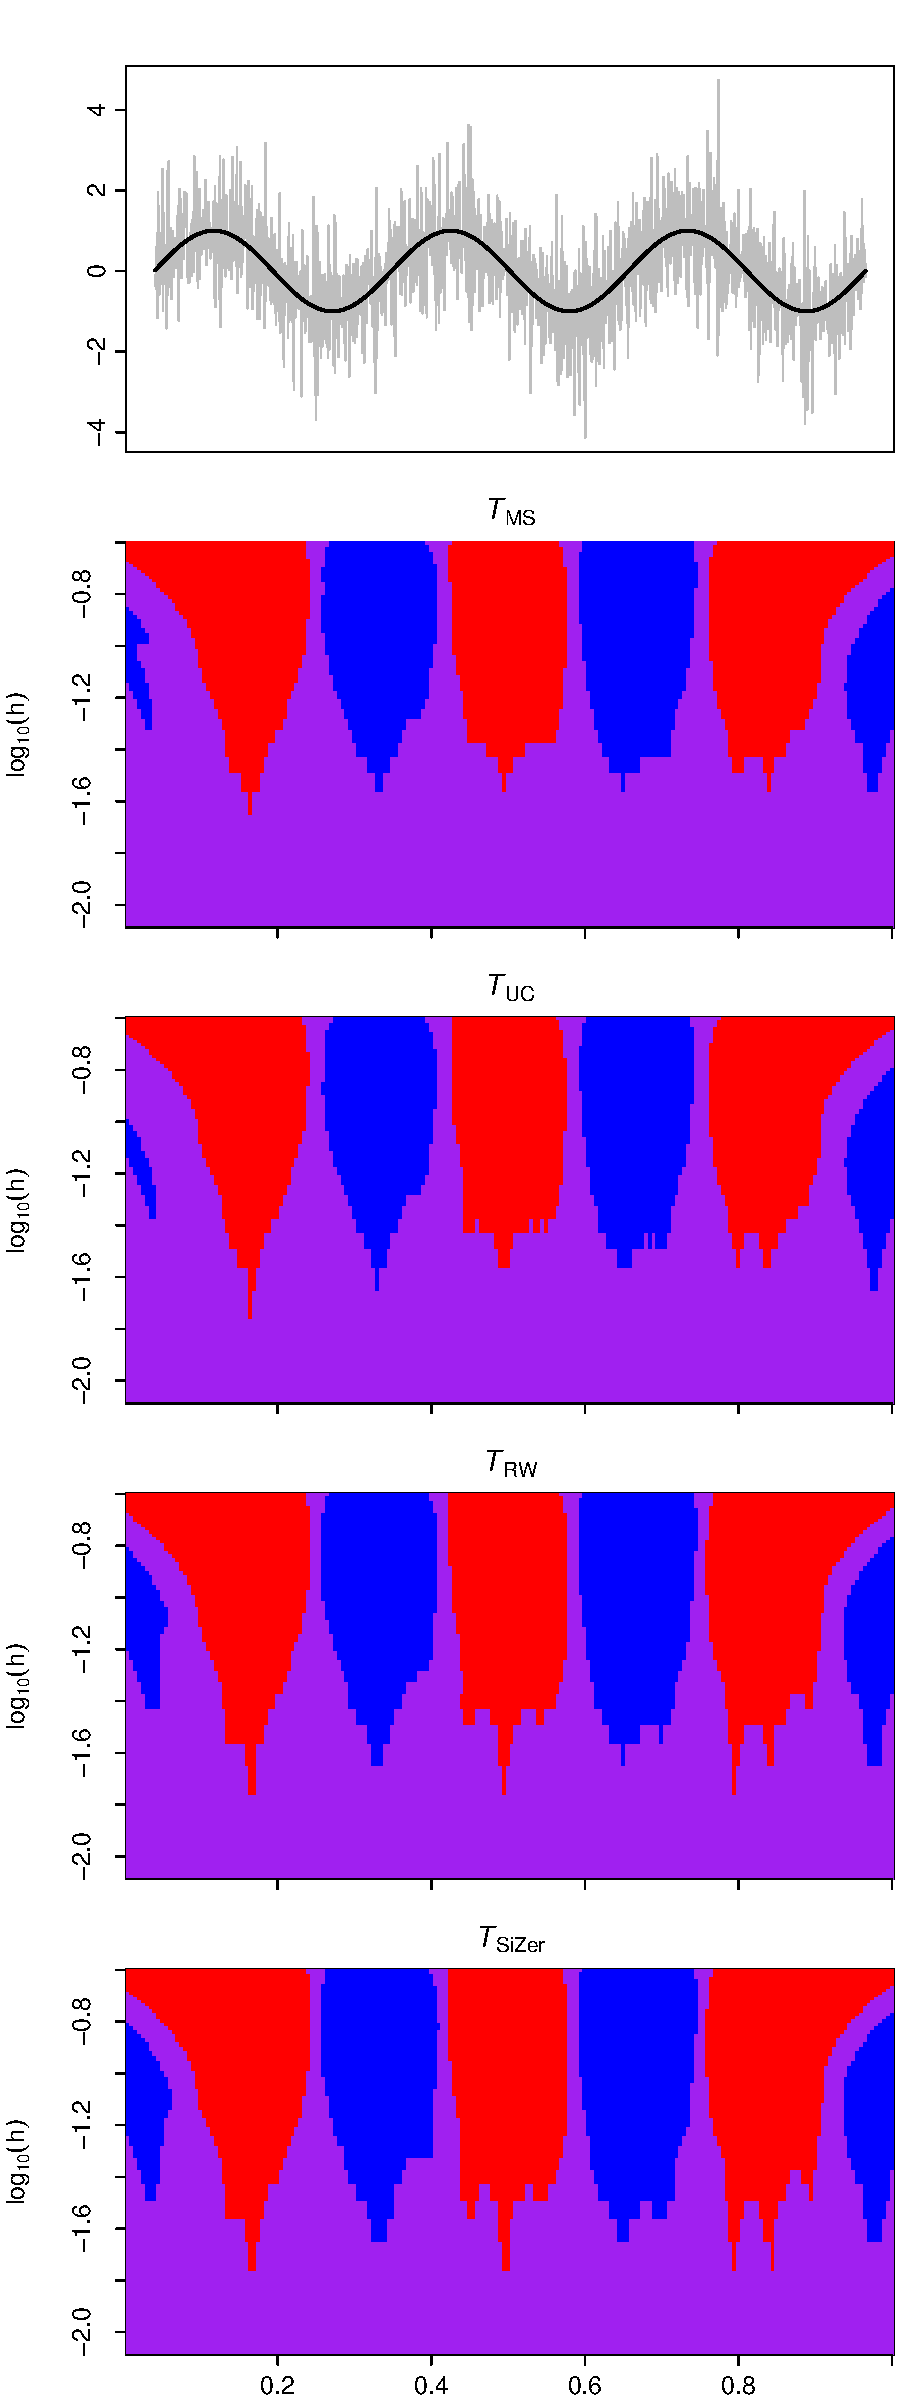
\includegraphics[width=\textwidth]{Plots/SiZermaps/SiZer_map_T_1000_sine_a1_-50_seed_1.pdf}
\caption{$a=-0.5$}
\end{subfigure}
\hspace{0.25cm}
\begin{subfigure}[b]{0.475\textwidth}
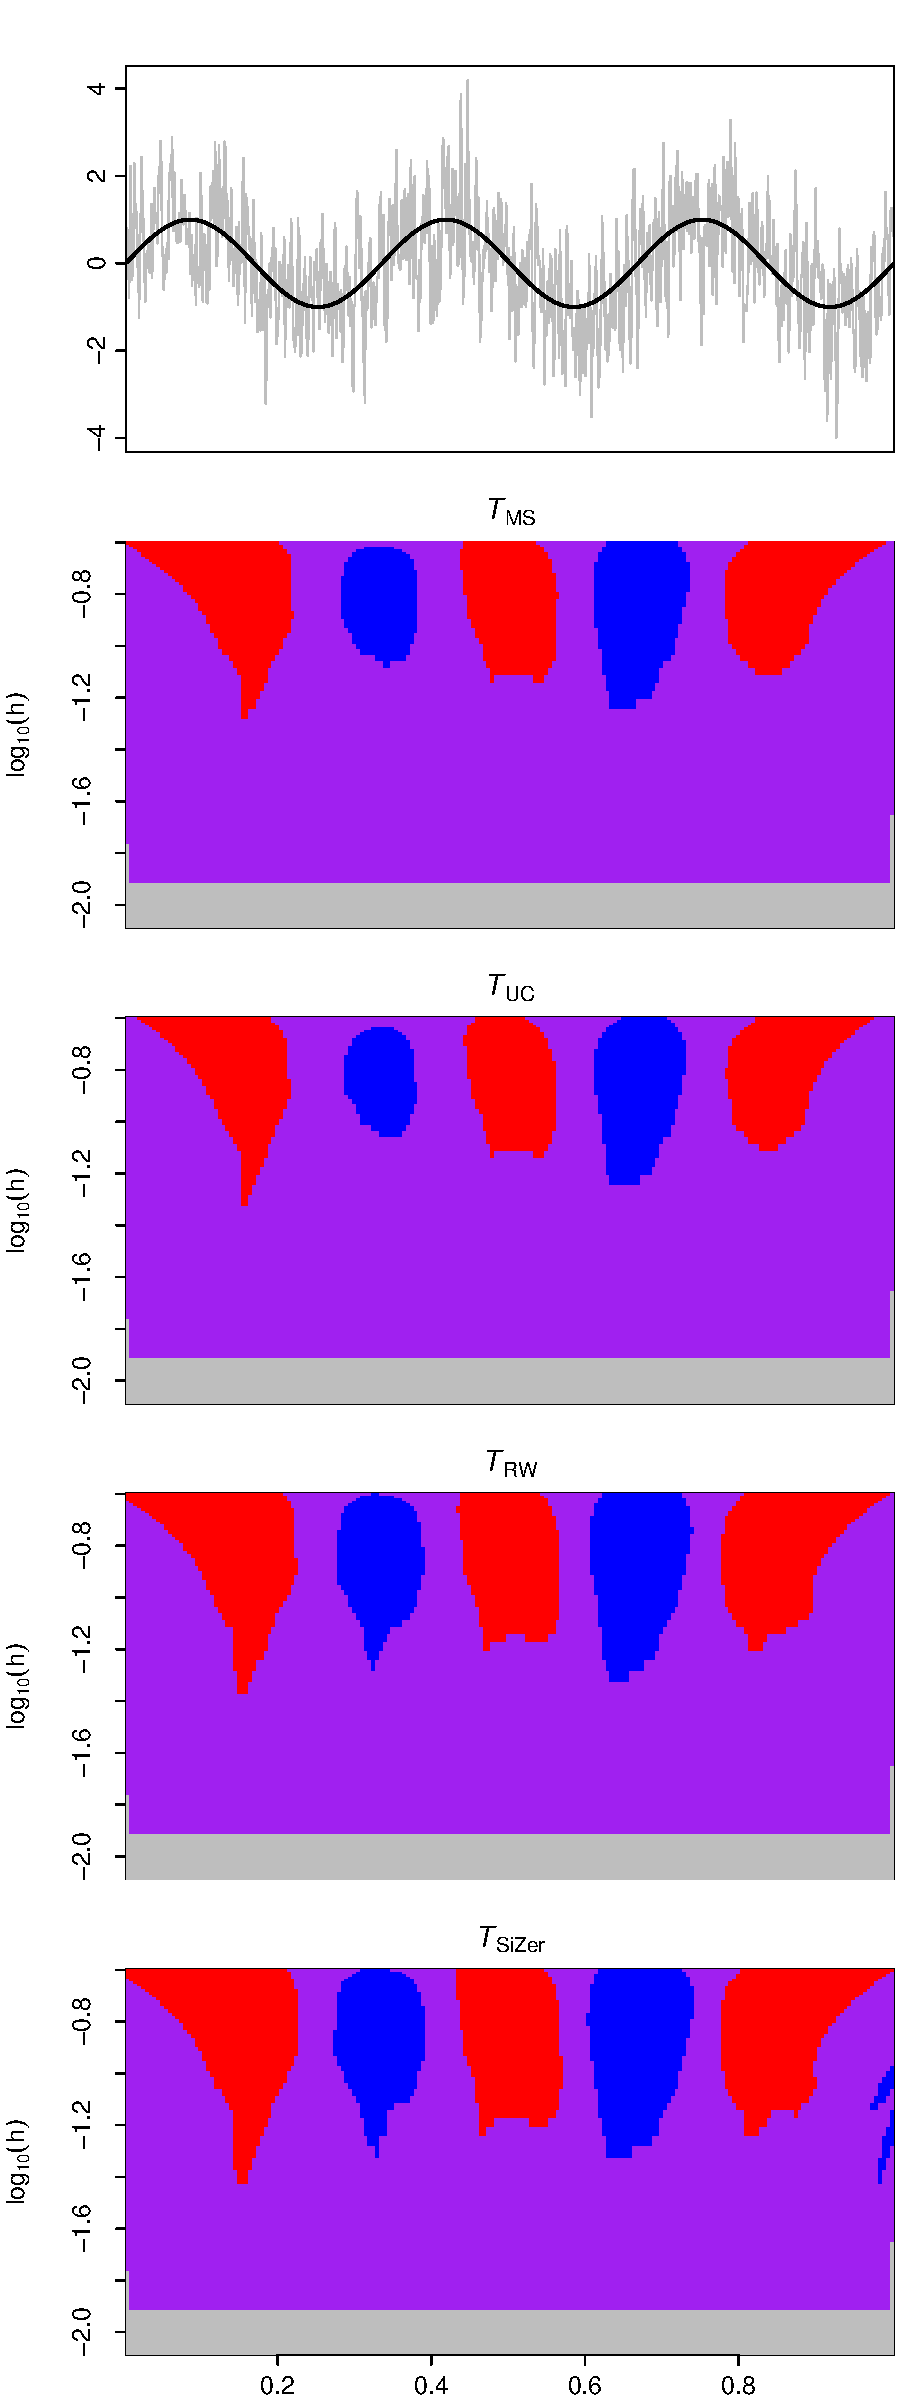
\includegraphics[width=\textwidth]{Plots/SiZermaps/SiZer_map_T_1000_sine_a1_50_seed_1.pdf}
\caption{$a=0.5$}
\end{subfigure}
\caption{SiZer maps for the sine example. The left-hand panels of subfigure (a) show the results for $a_1=-0.5$, the right-hand panels of subfigure (b) those for $a_1=0.5$. The two upper panels depicts the sine curve with the simulated data sample in the background. The other panels show the SiZer maps produced by the four tests $\mathcal{T}_{\text{MS}}$, $\mathcal{T}_{\text{UC}}$, $\mathcal{T}_{\text{RW}}$ and $\mathcal{T}_{\text{SiZer}}$.}\label{fig:sizer:sine}
\end{figure}  


\newpage
\subsection*{Robustness checks for Section \ref{subsec-sim-lrv}}


In what follows, we carry out some robustness checks to assess how sensitive the estimators $\widehat{a}$ and $\widehat{\sigma}^2$ are to the choice of the tuning parameters $q$ and $\overline{r}$. To do so, we repeat the simulation exercises of Section \ref{subsec-sim-lrv} for different values of $q$ and $\overline{r}$. In addition, we consider different choices of the tuning parameters $(m_1,m_2)$ on which the estimators of \cite{Hall2003} depend. As in Section \ref{subsec-sim-lrv}, we choose $m_1$ and $m_2$ such that $q$ lies between these values. We thus keep the parameters $q$ and $(m_1,m_2)$ roughly comparable. 


To start with, we consider the simulation scenarios with a moderate trend ($s_\beta = 1$). The MSE values of the estimators $\widehat{a}$, $\widehat{a}_{\text{HvK}}$, $\widehat{a}_{\text{oracle}}$ and $\widehat{\sigma}^2$, $\widehat{\sigma}^2_{\text{HvK}}$, $\widehat{\sigma}^2_{\text{oracle}}$ for these scenarios are presented in Figure \ref{fig:MSE_slope1} of Section \ref{subsec-sim-lrv}. These MSEs are re-calculated in Figures \ref{fig:MSE_slope1_AR_robust} and \ref{fig:MSE_slope1_lrv_robust} for a range of different choices of $q$, $\overline{r}$ and $(m_1,m_2)$. As one can see, the MSEs in the different plots of Figures \ref{fig:MSE_slope1_AR_robust} and \ref{fig:MSE_slope1_lrv_robust} are very similar. Hence, the MSE results reported in Section \ref{subsec-sim-lrv} for the scenarios with a moderate trend appear to be fairly robust to different choices of the tuning parameters. In particular, our estimators $\widehat{a}$ and $\widehat{\sigma}^2$ seem to be quite insensitive to the choice of tuning parameters, at least as far as their MSEs are concerned.


We next turn to the simulation designs with a pronounced trend ($s_\beta = 10$). The MSE values of the estimators in these scenarios are reported in Figure \ref{fig:MSE_slope10} of Section \ref{subsec-sim-lrv}. Analogously as before, we re-calculate these MSEs for different tuning parameters in Figures \ref{fig:MSE_slope10_AR_robust}--\ref{fig:MSE_slope10_lrv_robust}. Figure \ref{fig:MSE_slope10_AR_zoom_robust} is a zoomed-in version of Figure \ref{fig:MSE_slope10_AR_robust} which is added for better visibility. As can be seen, our estimators appear to be barely influenced by the choice of $q$. However, the MSE values become somewhat larger when $\overline{r}$ is chosen bigger. This is of course not very surprising: The main reason why the estimator $\widehat{a}$ works well in the presence of a strong trend is that it is only based on differences of small orders. If we increase $\overline{r}$, we use larger differences to compute $\widehat{a}$, which results in not eliminating the trend $m$ appropriately any more. This becomes visible in somewhat larger MSE values. Nevertheless, overall, our estimators appear not to be strongly influenced by the choice of tuning parameters (in terms of MSE) as long as these are chosen within reasonable bounds. 


\begin{figure}[h!]
\begin{subfigure}[b]{0.45\textwidth}
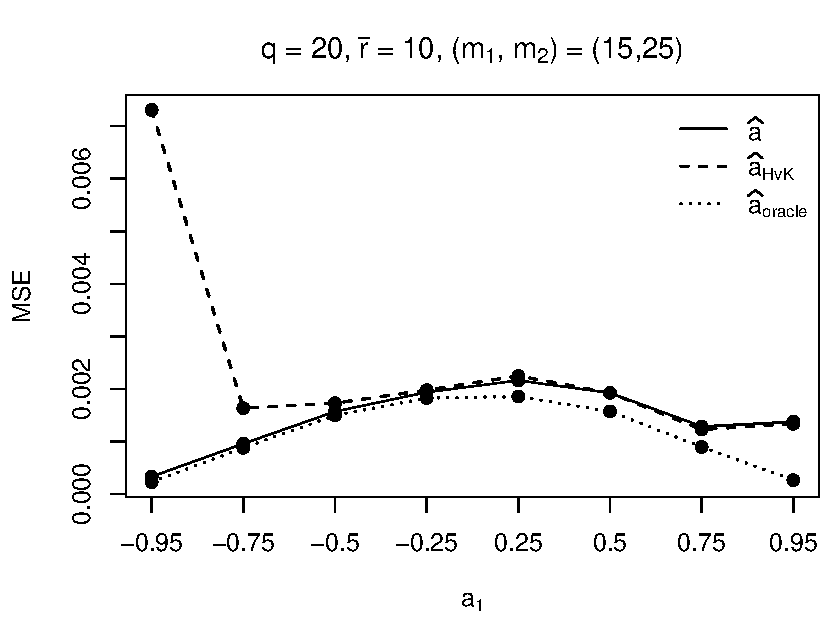
\includegraphics[width=\textwidth]{Plots/Robustness/MSE_a1_T=500_slope=1_(q,r,M1,M2)=(20,10,15,25).pdf}
\end{subfigure}
\hspace{0.25cm}
\begin{subfigure}[b]{0.45\textwidth}
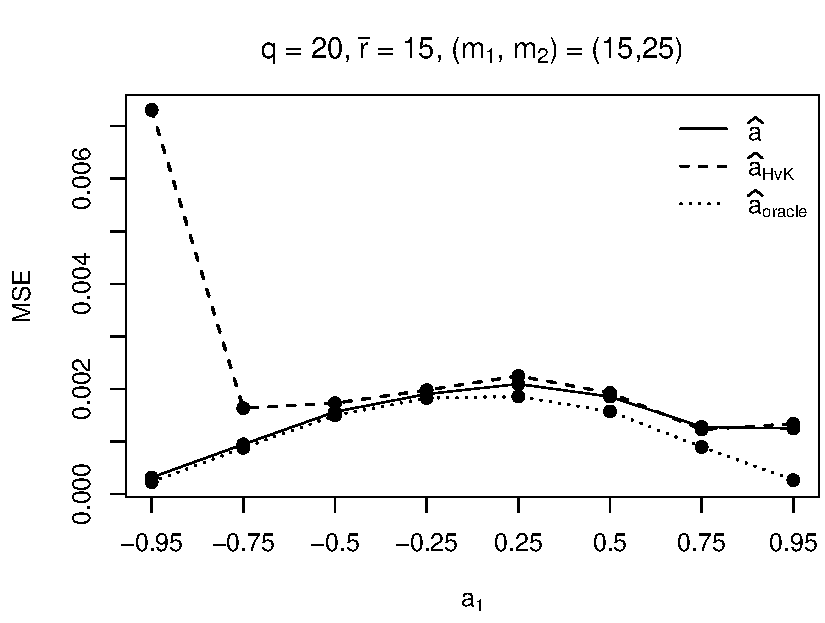
\includegraphics[width=\textwidth]{Plots/Robustness/MSE_a1_T=500_slope=1_(q,r,M1,M2)=(20,15,15,25).pdf}
\end{subfigure}

\begin{subfigure}[b]{0.45\textwidth}
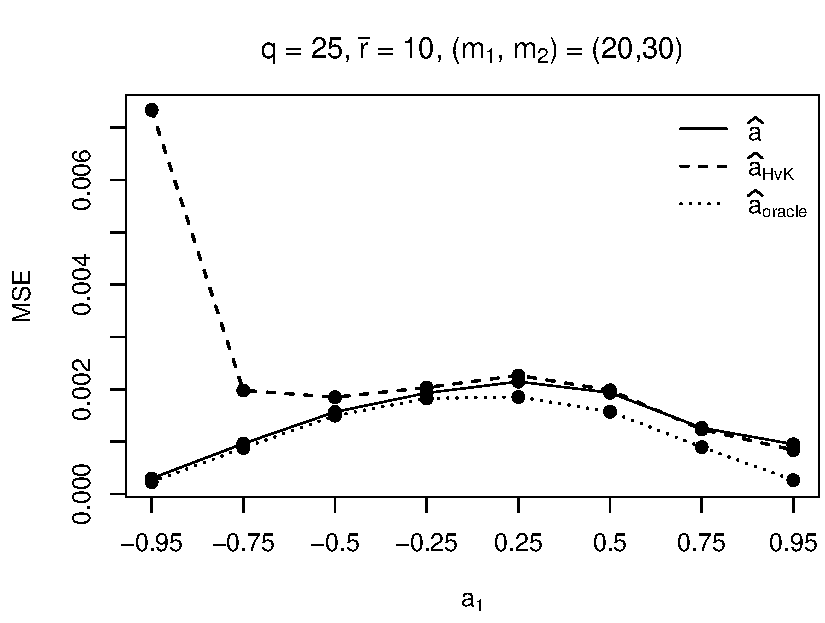
\includegraphics[width=\textwidth]{Plots/Robustness/MSE_a1_T=500_slope=1_(q,r,M1,M2)=(25,10,20,30).pdf}
\end{subfigure}
\hspace{0.25cm}
\begin{subfigure}[b]{0.45\textwidth}
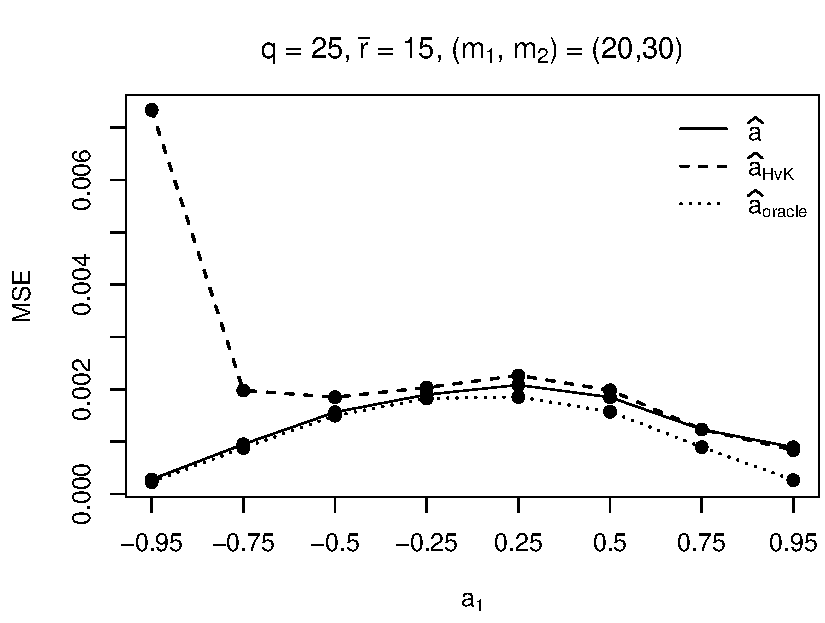
\includegraphics[width=\textwidth]{Plots/Robustness/MSE_a1_T=500_slope=1_(q,r,M1,M2)=(25,15,20,30).pdf}
\end{subfigure}

\begin{subfigure}[b]{0.45\textwidth}
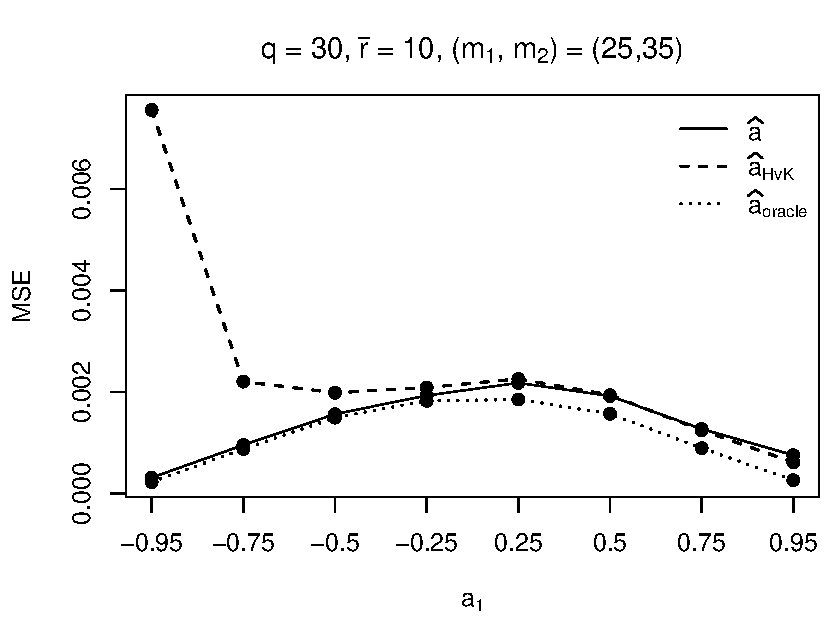
\includegraphics[width=\textwidth]{Plots/Robustness/MSE_a1_T=500_slope=1_(q,r,M1,M2)=(30,10,25,35).pdf}
\end{subfigure}
\hspace{0.25cm}
\begin{subfigure}[b]{0.45\textwidth}
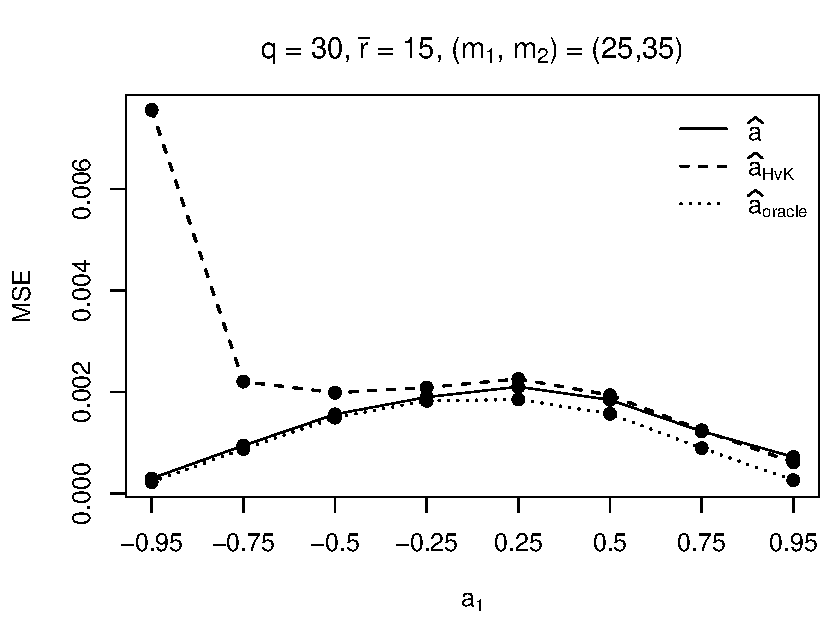
\includegraphics[width=\textwidth]{Plots/Robustness/MSE_a1_T=500_slope=1_(q,r,M1,M2)=(30,15,25,35).pdf}
\end{subfigure}

\begin{subfigure}[b]{0.45\textwidth}
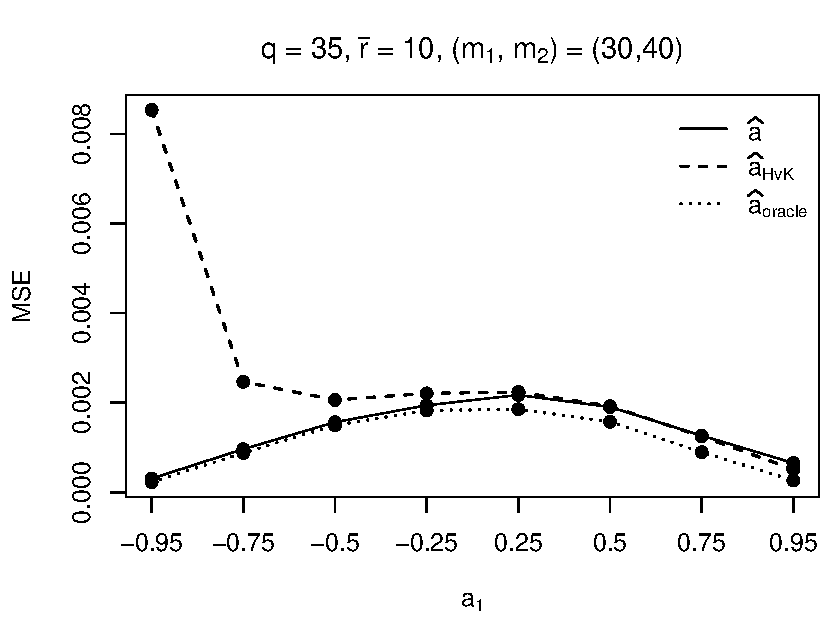
\includegraphics[width=\textwidth]{Plots/Robustness/MSE_a1_T=500_slope=1_(q,r,M1,M2)=(35,10,30,40).pdf}
\end{subfigure}
\hspace{0.25cm}
\begin{subfigure}[b]{0.45\textwidth}
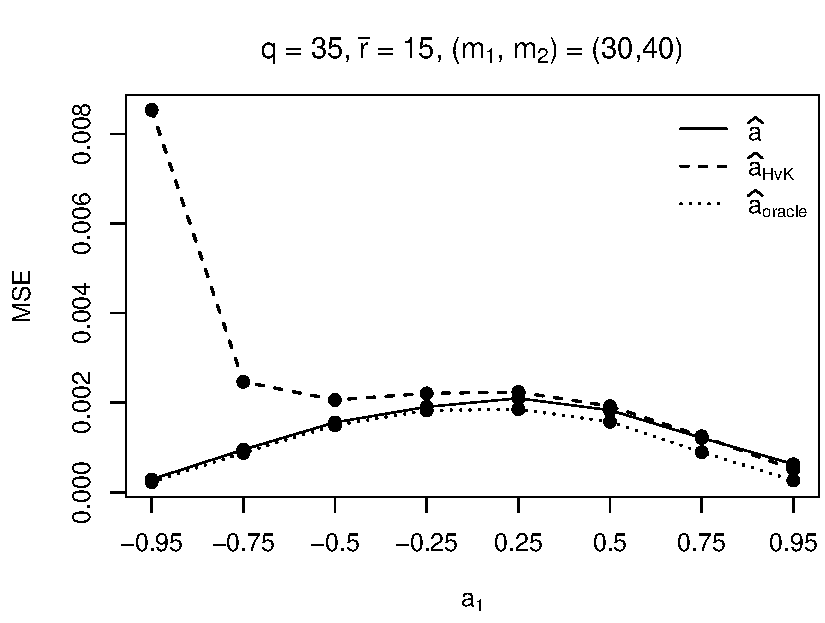
\includegraphics[width=\textwidth]{Plots/Robustness/MSE_a1_T=500_slope=1_(q,r,M1,M2)=(35,15,30,40).pdf}
\end{subfigure}
\caption{MSE values for the estimators $\widehat{a}$, $\widehat{a}_{\text{HvK}}$ and $\widehat{a}_{\text{oracle}}$ in the scenario with a moderate trend ($s_\beta=1$).}\label{fig:MSE_slope1_AR_robust} 
\end{figure}


\begin{figure}[p]
\begin{subfigure}[b]{0.45\textwidth}
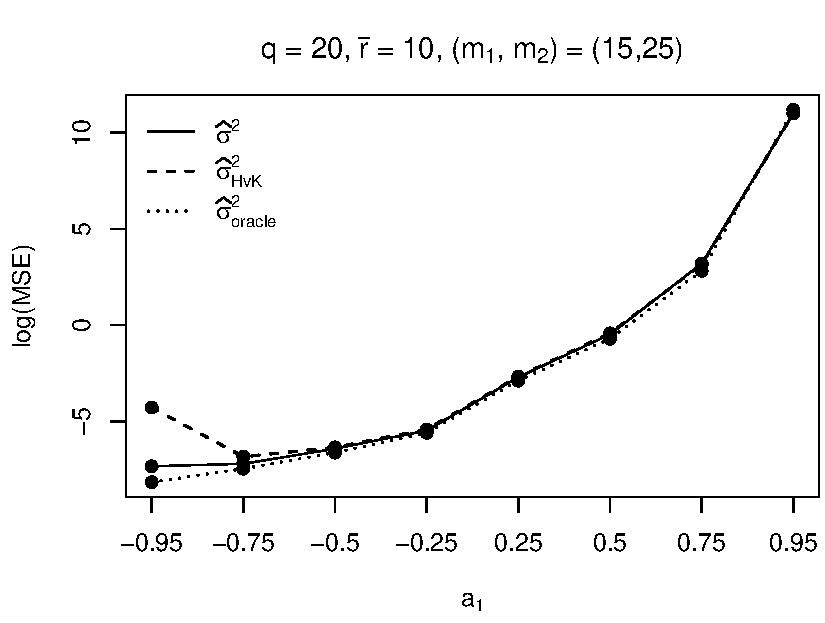
\includegraphics[width=\textwidth]{Plots/Robustness/MSE_lrv_T=500_slope=1_(q,r,M1,M2)=(20,10,15,25).pdf}
\end{subfigure}
\hspace{0.25cm}
\begin{subfigure}[b]{0.45\textwidth}
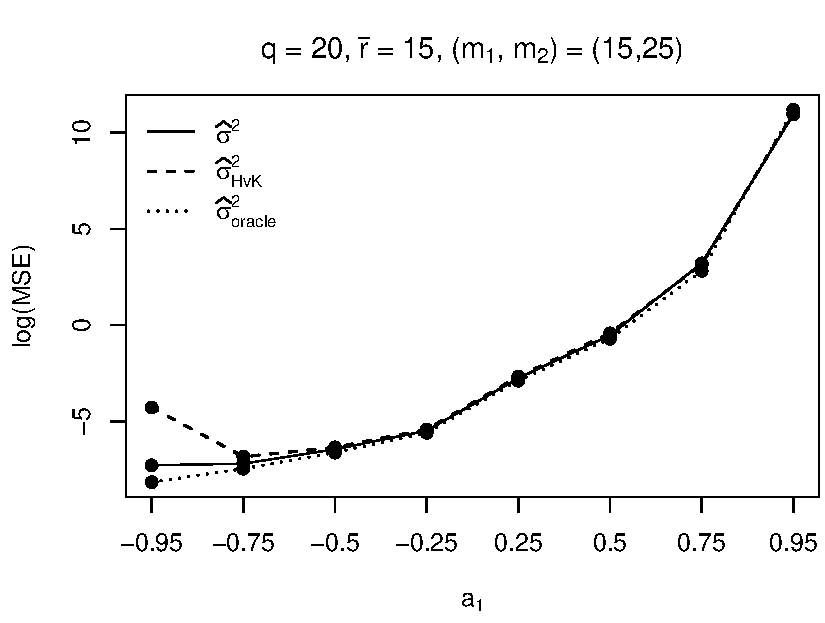
\includegraphics[width=\textwidth]{Plots/Robustness/MSE_lrv_T=500_slope=1_(q,r,M1,M2)=(20,15,15,25).pdf}
\end{subfigure}

\begin{subfigure}[b]{0.45\textwidth}
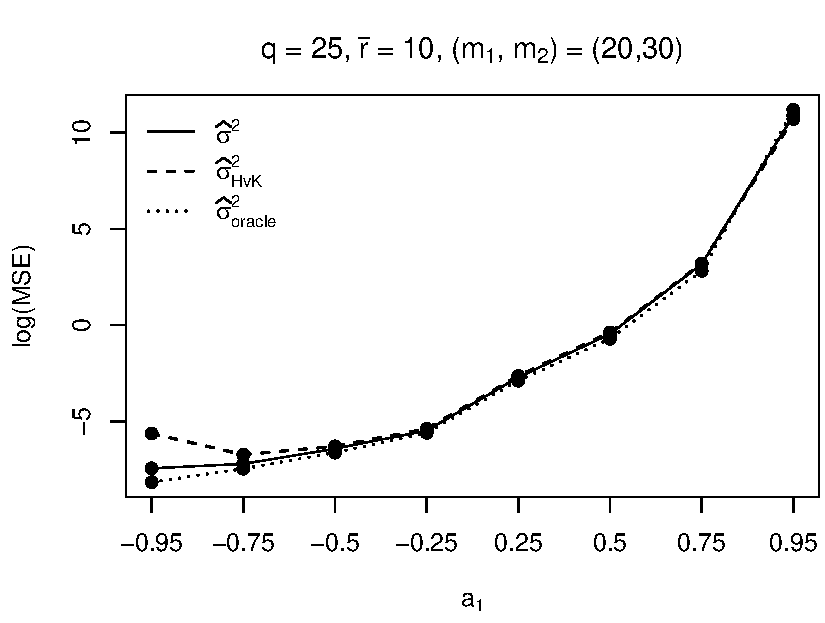
\includegraphics[width=\textwidth]{Plots/Robustness/MSE_lrv_T=500_slope=1_(q,r,M1,M2)=(25,10,20,30).pdf}
\end{subfigure}
\hspace{0.25cm}
\begin{subfigure}[b]{0.45\textwidth}
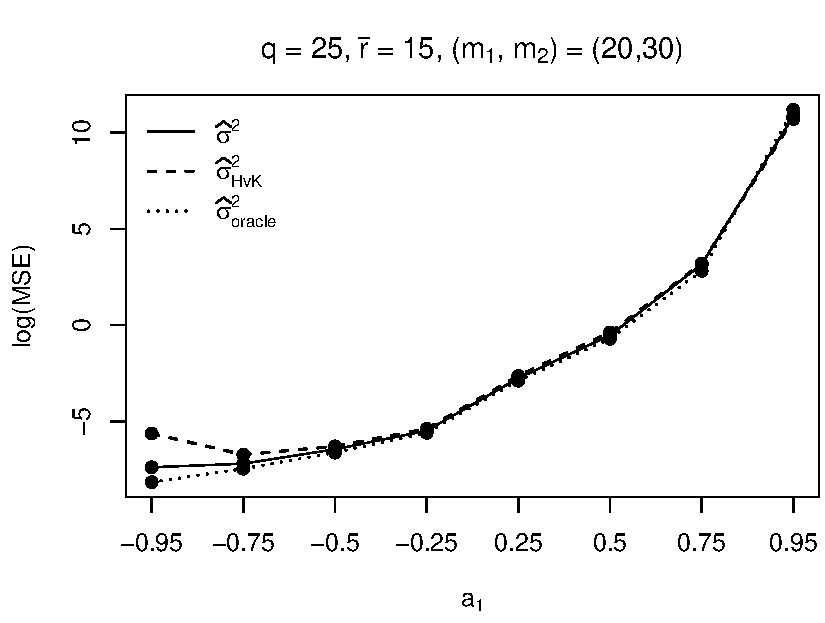
\includegraphics[width=\textwidth]{Plots/Robustness/MSE_lrv_T=500_slope=1_(q,r,M1,M2)=(25,15,20,30).pdf}
\end{subfigure}

\begin{subfigure}[b]{0.45\textwidth}
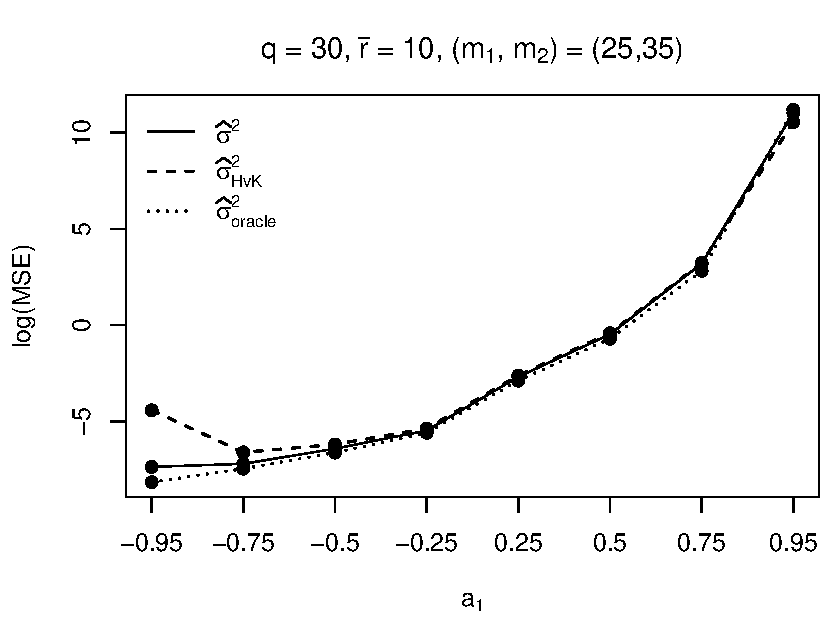
\includegraphics[width=\textwidth]{Plots/Robustness/MSE_lrv_T=500_slope=1_(q,r,M1,M2)=(30,10,25,35).pdf}
\end{subfigure}
\hspace{0.25cm}
\begin{subfigure}[b]{0.45\textwidth}
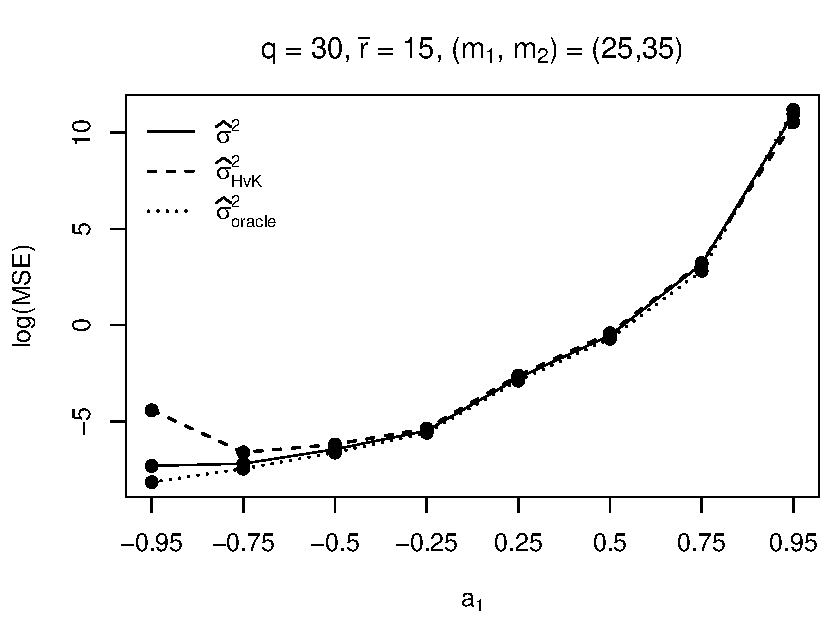
\includegraphics[width=\textwidth]{Plots/Robustness/MSE_lrv_T=500_slope=1_(q,r,M1,M2)=(30,15,25,35).pdf}
\end{subfigure}

\begin{subfigure}[b]{0.45\textwidth}
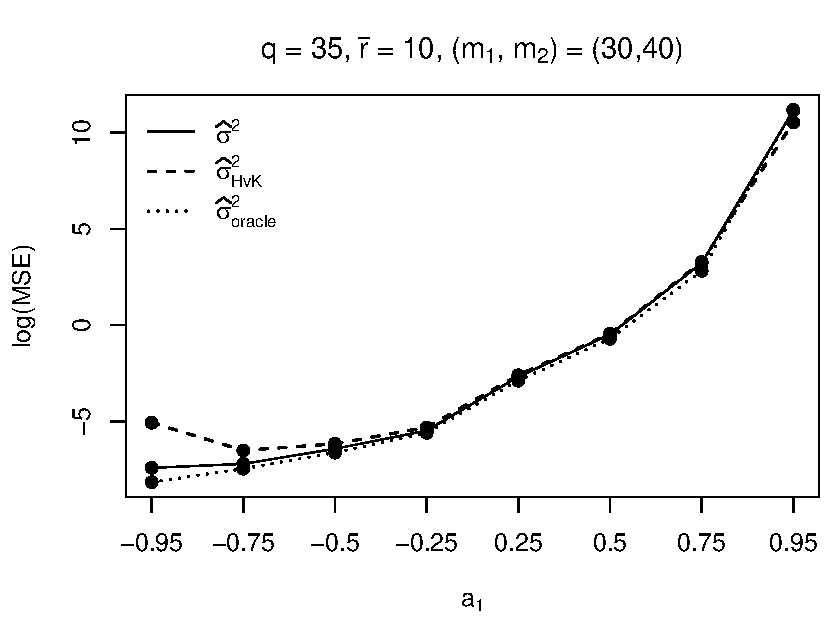
\includegraphics[width=\textwidth]{Plots/Robustness/MSE_lrv_T=500_slope=1_(q,r,M1,M2)=(35,10,30,40).pdf}
\end{subfigure}
\hspace{0.25cm}
\begin{subfigure}[b]{0.45\textwidth}
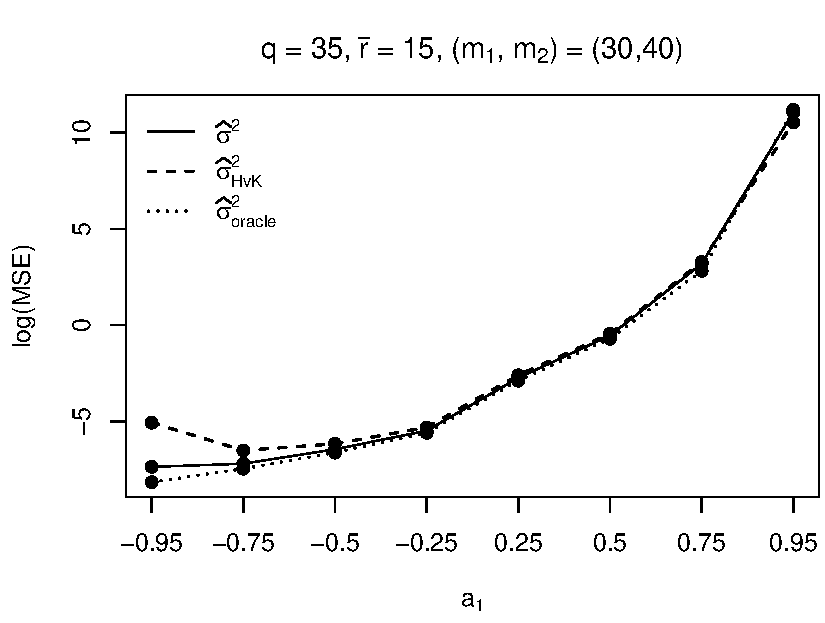
\includegraphics[width=\textwidth]{Plots/Robustness/MSE_lrv_T=500_slope=1_(q,r,M1,M2)=(35,15,30,40).pdf}
\end{subfigure}
\caption{Logarithmic MSE values for the estimators $\widehat{\sigma}^2$, $\widehat{\sigma}^2_{\text{HvK}}$ and $\widehat{\sigma}^2_{\text{oracle}}$ in the scenario with a moderate trend ($s_\beta=1$).}\label{fig:MSE_slope1_lrv_robust}
\end{figure}


\begin{figure}[p]
\begin{subfigure}[b]{0.45\textwidth}
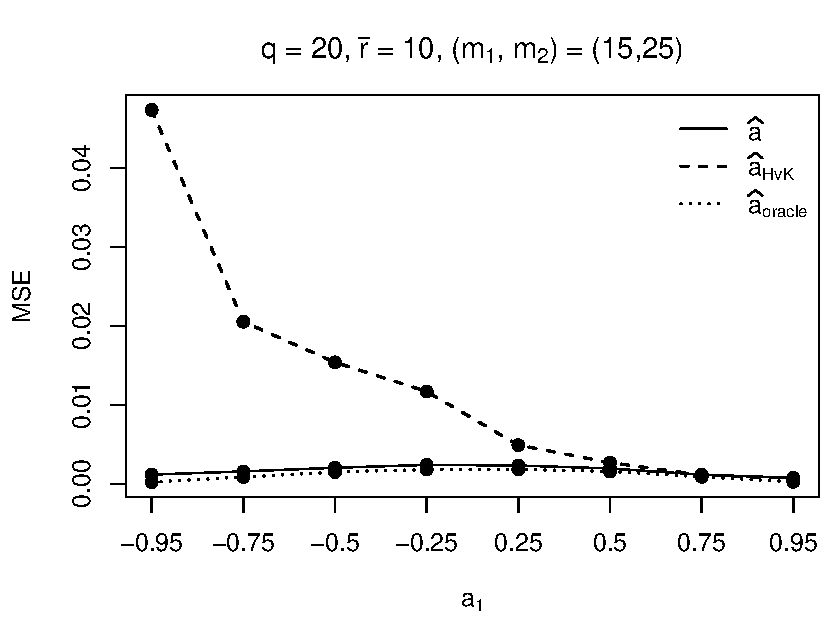
\includegraphics[width=\textwidth]{Plots/Robustness/MSE_a1_T=500_slope=10_(q,r,M1,M2)=(20,10,15,25).pdf}
\end{subfigure}
\hspace{0.25cm}
\begin{subfigure}[b]{0.45\textwidth}
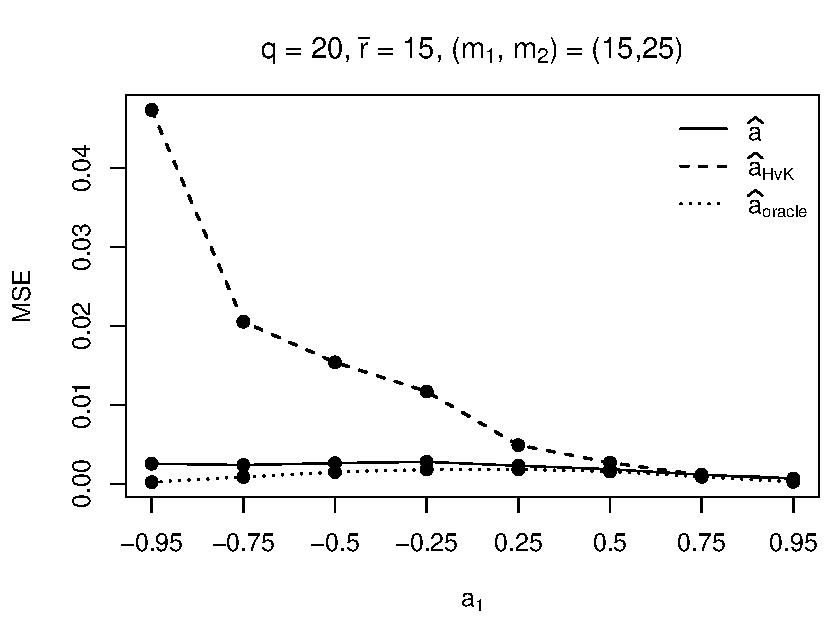
\includegraphics[width=\textwidth]{Plots/Robustness/MSE_a1_T=500_slope=10_(q,r,M1,M2)=(20,15,15,25).pdf}
\end{subfigure}

\begin{subfigure}[b]{0.45\textwidth}
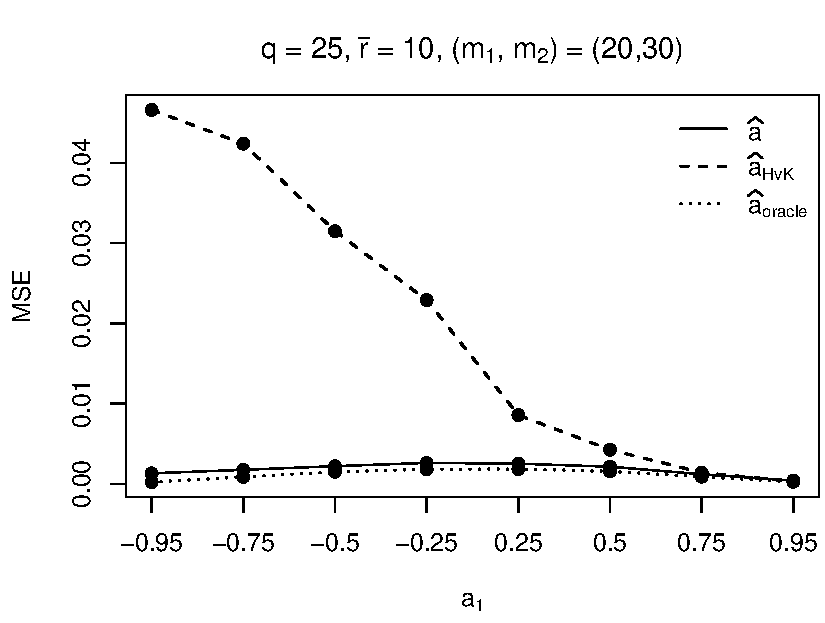
\includegraphics[width=\textwidth]{Plots/Robustness/MSE_a1_T=500_slope=10_(q,r,M1,M2)=(25,10,20,30).pdf}
\end{subfigure}
\hspace{0.25cm}
\begin{subfigure}[b]{0.45\textwidth}
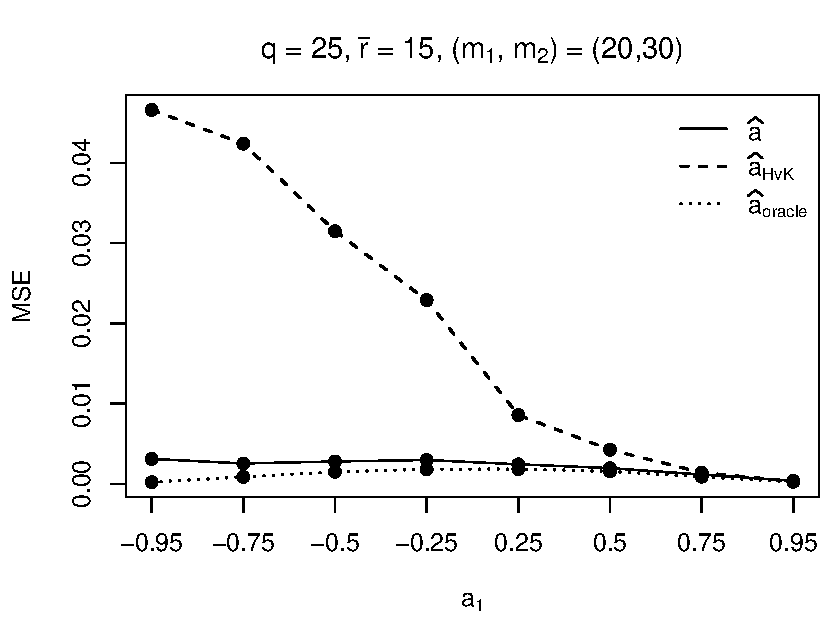
\includegraphics[width=\textwidth]{Plots/Robustness/MSE_a1_T=500_slope=10_(q,r,M1,M2)=(25,15,20,30).pdf}
\end{subfigure}

\begin{subfigure}[b]{0.45\textwidth}
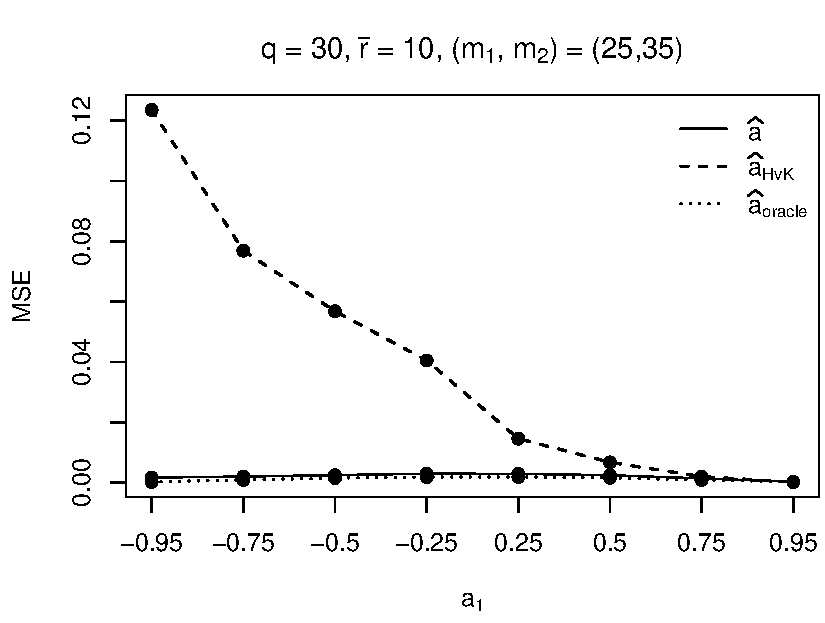
\includegraphics[width=\textwidth]{Plots/Robustness/MSE_a1_T=500_slope=10_(q,r,M1,M2)=(30,10,25,35).pdf}
\end{subfigure}
\hspace{0.25cm}
\begin{subfigure}[b]{0.45\textwidth}
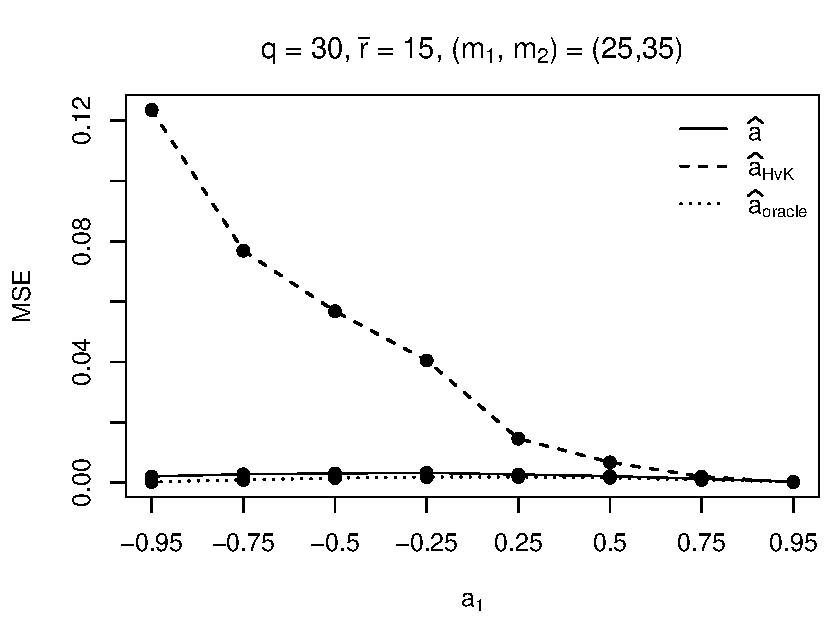
\includegraphics[width=\textwidth]{Plots/Robustness/MSE_a1_T=500_slope=10_(q,r,M1,M2)=(30,15,25,35).pdf}
\end{subfigure}

\begin{subfigure}[b]{0.45\textwidth}
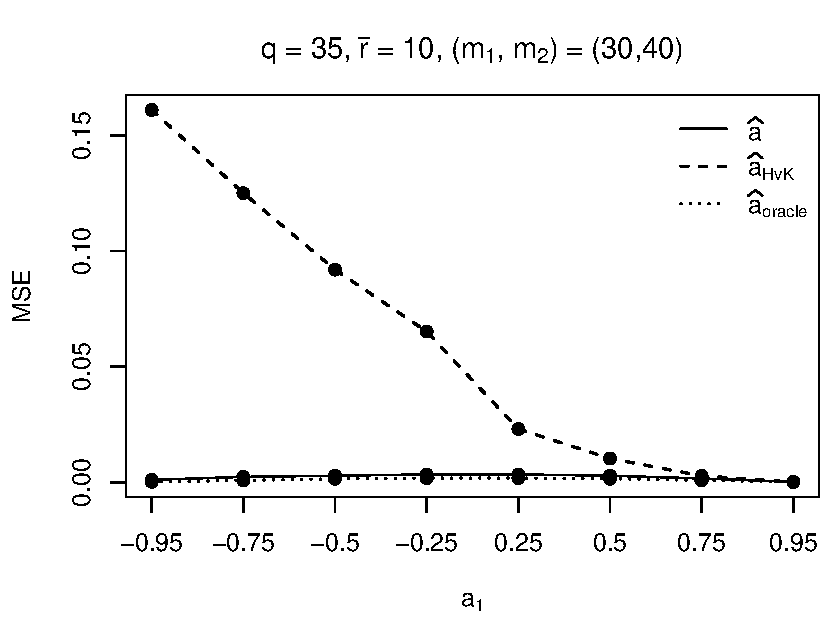
\includegraphics[width=\textwidth]{Plots/Robustness/MSE_a1_T=500_slope=10_(q,r,M1,M2)=(35,10,30,40).pdf}
\end{subfigure}
\hspace{0.25cm}
\begin{subfigure}[b]{0.45\textwidth}
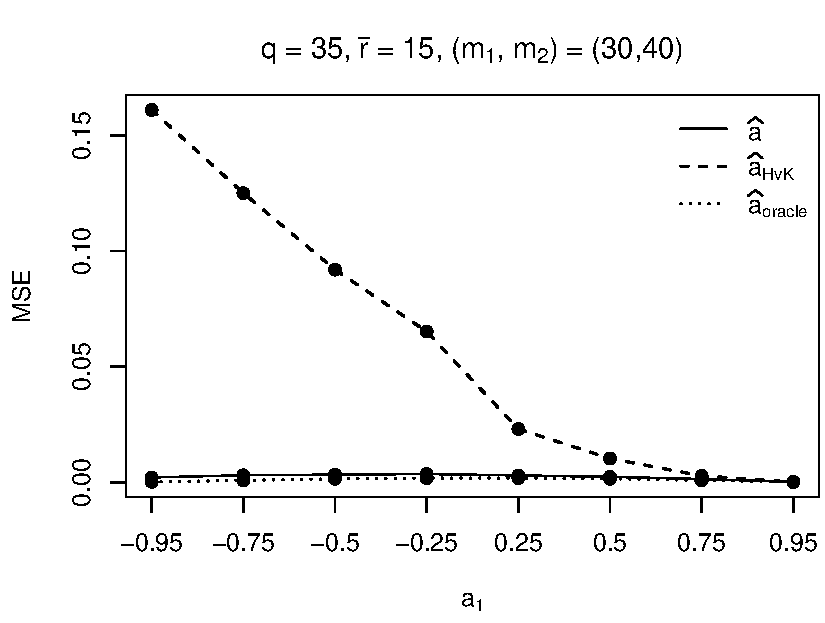
\includegraphics[width=\textwidth]{Plots/Robustness/MSE_a1_T=500_slope=10_(q,r,M1,M2)=(35,15,30,40).pdf}
\end{subfigure}
\caption{MSE values for the estimators $\widehat{a}$, $\widehat{a}_{\text{HvK}}$ and $\widehat{a}_{\text{oracle}}$ in the scenario with a pronounced trend ($s_\beta=10$).}\label{fig:MSE_slope10_AR_robust} 
\end{figure}


\begin{figure}[p]
\begin{subfigure}[b]{0.45\textwidth}
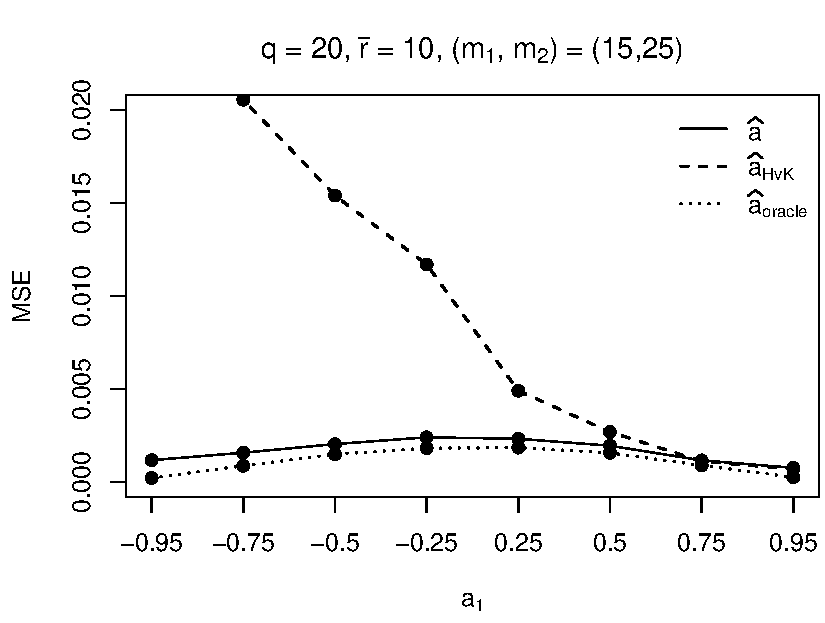
\includegraphics[width=\textwidth]{Plots/Robustness/MSE_a1_zoomed_T=500_slope=10_(q,r,M1,M2)=(20,10,15,25).pdf}
\end{subfigure}
\hspace{0.25cm}
\begin{subfigure}[b]{0.45\textwidth}
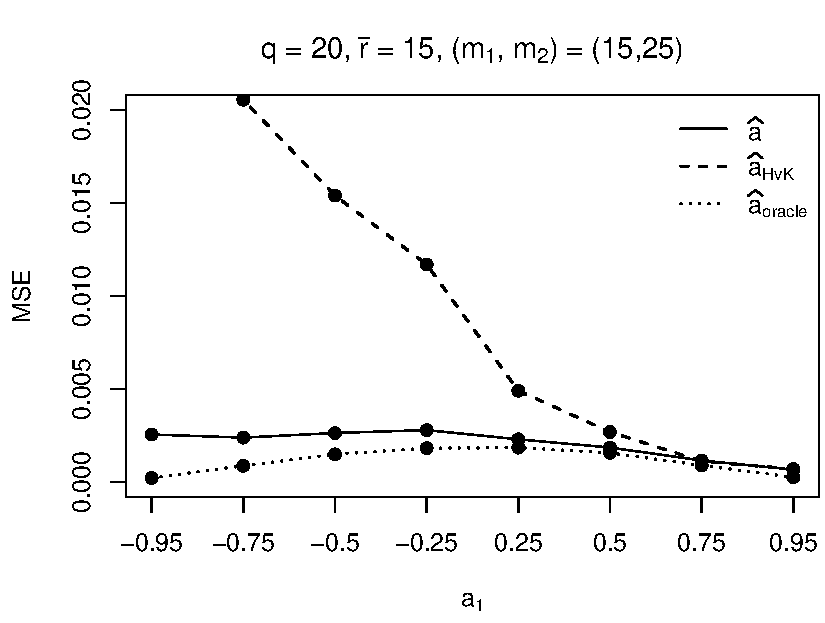
\includegraphics[width=\textwidth]{Plots/Robustness/MSE_a1_zoomed_T=500_slope=10_(q,r,M1,M2)=(20,15,15,25).pdf}
\end{subfigure}

\begin{subfigure}[b]{0.45\textwidth}
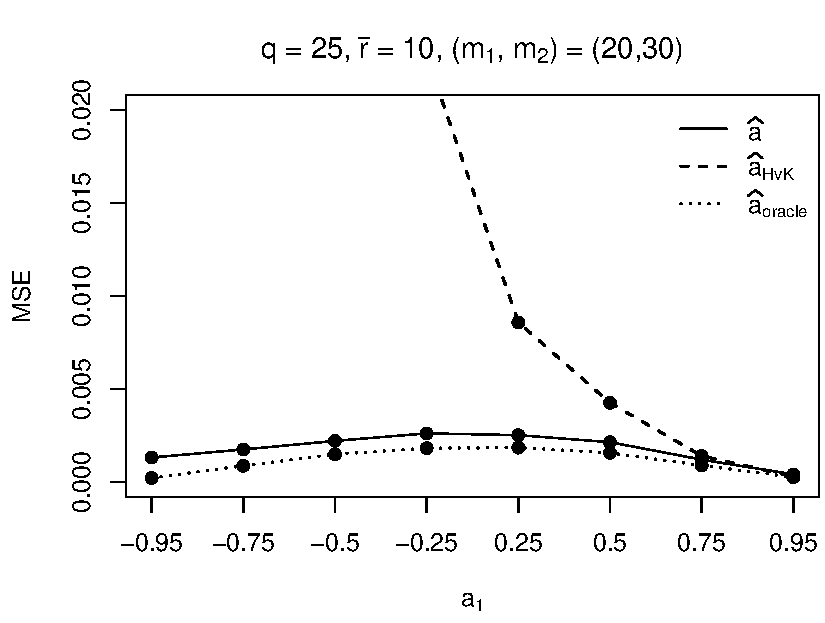
\includegraphics[width=\textwidth]{Plots/Robustness/MSE_a1_zoomed_T=500_slope=10_(q,r,M1,M2)=(25,10,20,30).pdf}
\end{subfigure}
\hspace{0.25cm}
\begin{subfigure}[b]{0.45\textwidth}
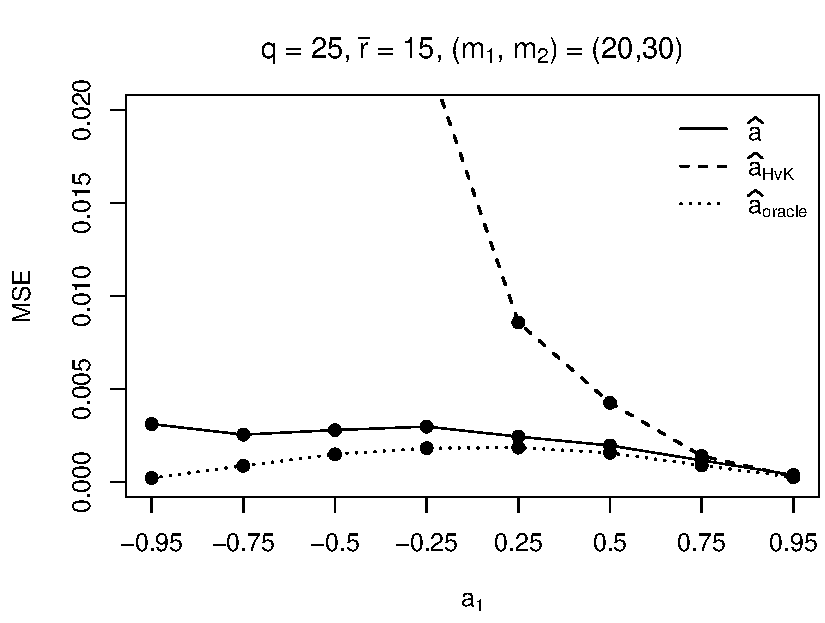
\includegraphics[width=\textwidth]{Plots/Robustness/MSE_a1_zoomed_T=500_slope=10_(q,r,M1,M2)=(25,15,20,30).pdf}
\end{subfigure}

\begin{subfigure}[b]{0.45\textwidth}
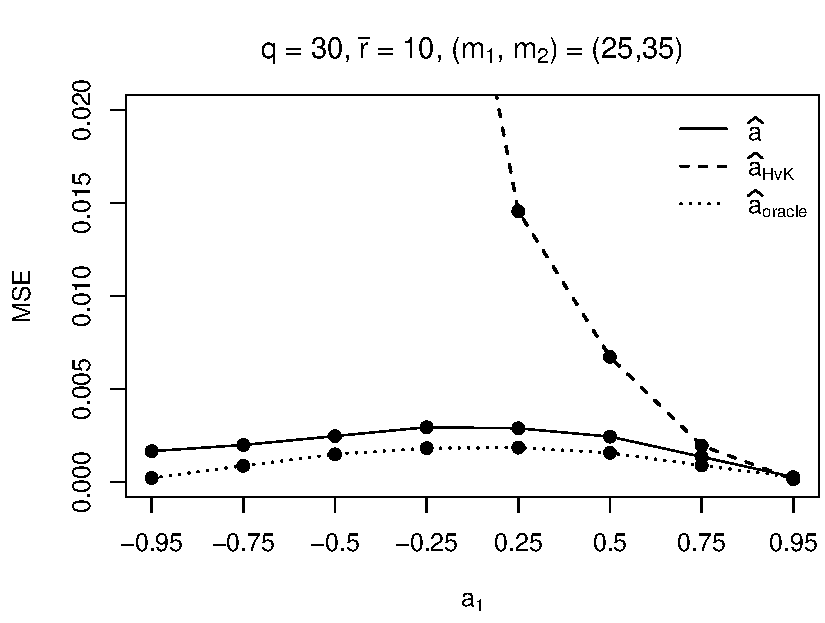
\includegraphics[width=\textwidth]{Plots/Robustness/MSE_a1_zoomed_T=500_slope=10_(q,r,M1,M2)=(30,10,25,35).pdf}
\end{subfigure}
\hspace{0.25cm}
\begin{subfigure}[b]{0.45\textwidth}
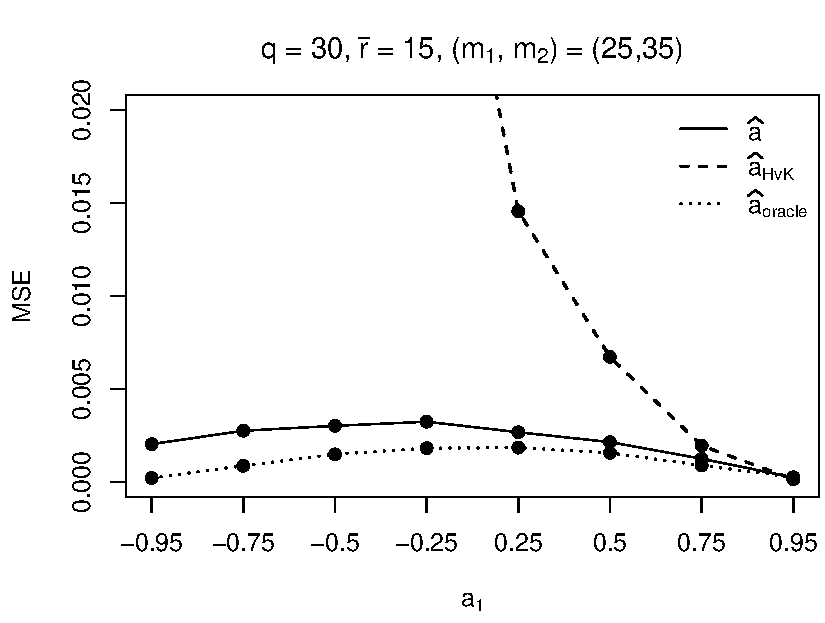
\includegraphics[width=\textwidth]{Plots/Robustness/MSE_a1_zoomed_T=500_slope=10_(q,r,M1,M2)=(30,15,25,35).pdf}
\end{subfigure}

\begin{subfigure}[b]{0.45\textwidth}
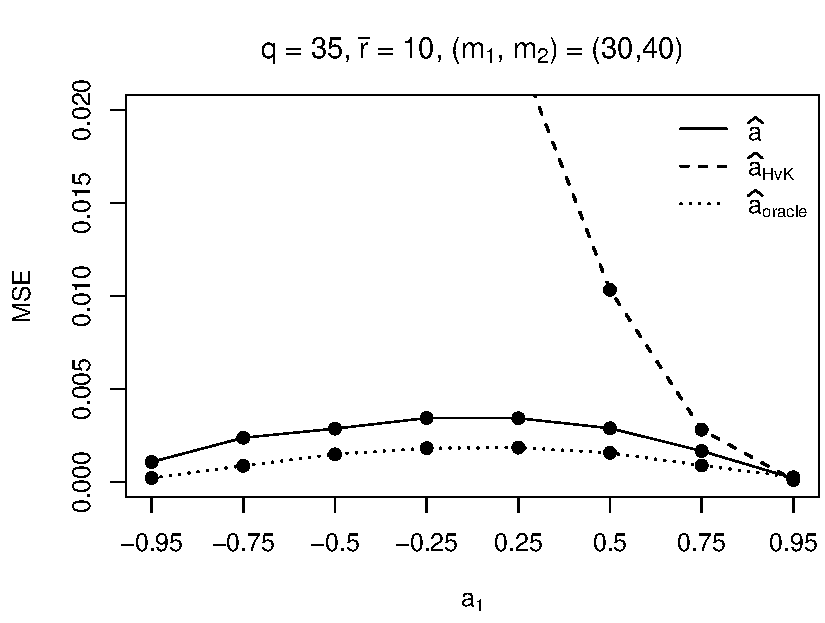
\includegraphics[width=\textwidth]{Plots/Robustness/MSE_a1_zoomed_T=500_slope=10_(q,r,M1,M2)=(35,10,30,40).pdf}
\end{subfigure}
\hspace{0.25cm}
\begin{subfigure}[b]{0.45\textwidth}
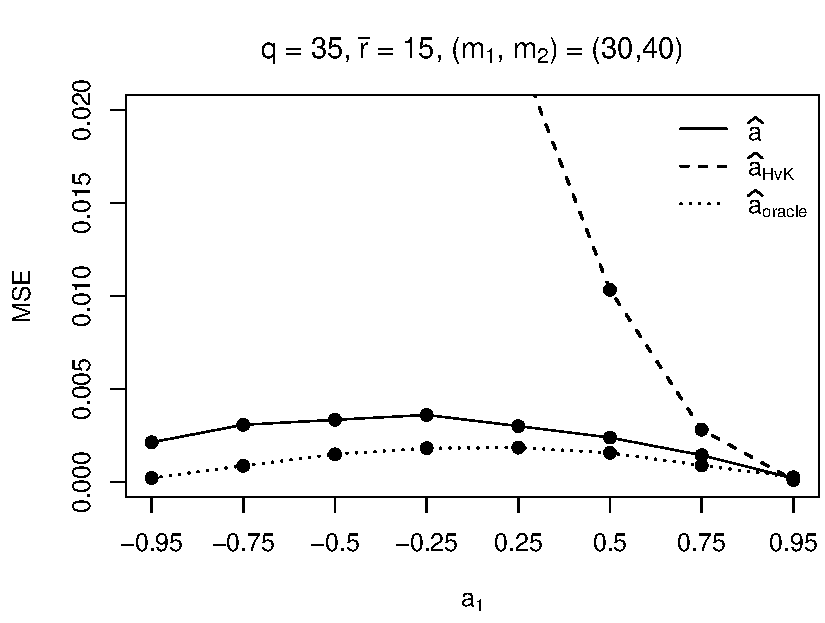
\includegraphics[width=\textwidth]{Plots/Robustness/MSE_a1_zoomed_T=500_slope=10_(q,r,M1,M2)=(35,15,30,40).pdf}
\end{subfigure}
\caption{MSE values for the estimators $\widehat{a}$, $\widehat{a}_{\text{HvK}}$ and $\widehat{a}_{\text{oracle}}$ in the scenario with a pronounced trend ($s_\beta=10$). The plots are zoomed-in versions of the respective plots in Figure \ref{fig:MSE_slope10_AR_robust}.}\label{fig:MSE_slope10_AR_zoom_robust}
\end{figure}


\begin{figure}[p]
\begin{subfigure}[b]{0.45\textwidth}
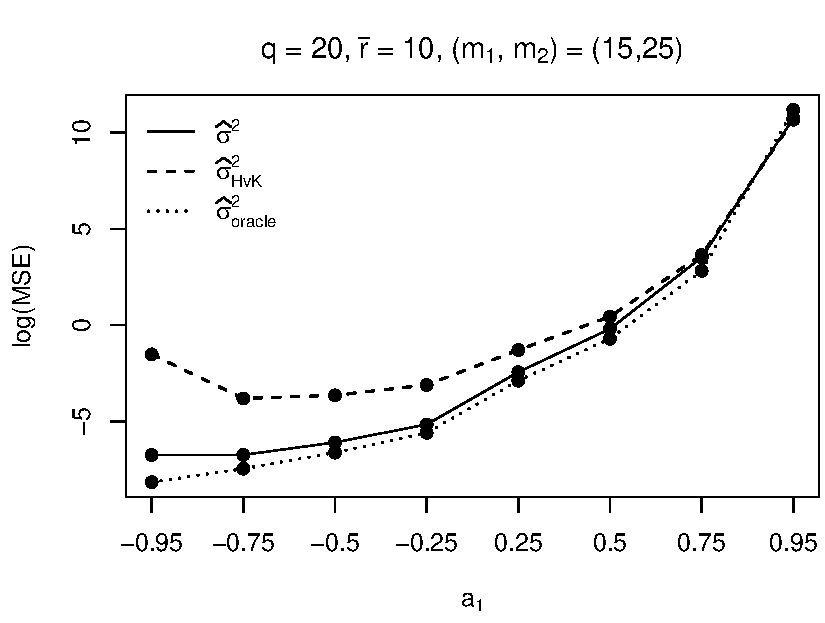
\includegraphics[width=\textwidth]{Plots/Robustness/MSE_lrv_T=500_slope=10_(q,r,M1,M2)=(20,10,15,25).pdf}
\end{subfigure}
\hspace{0.25cm}
\begin{subfigure}[b]{0.45\textwidth}
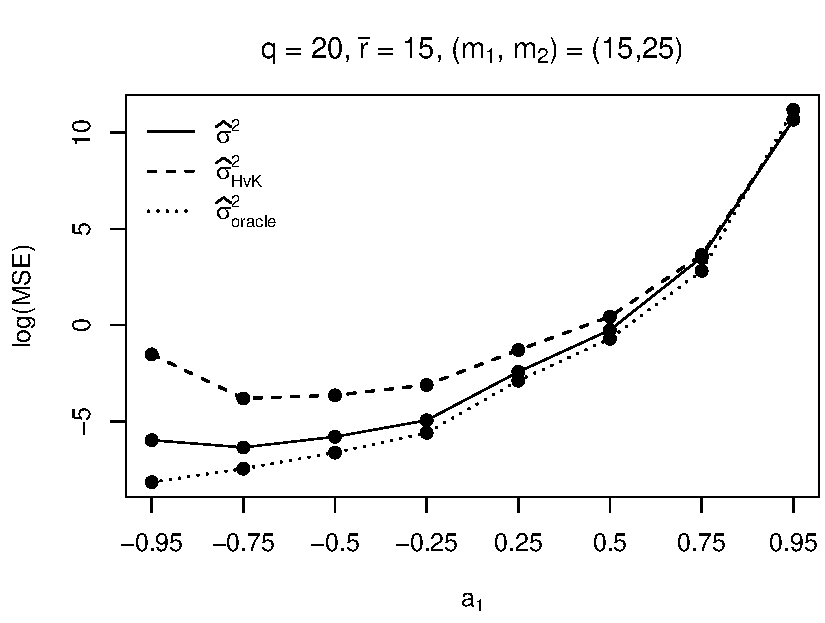
\includegraphics[width=\textwidth]{Plots/Robustness/MSE_lrv_T=500_slope=10_(q,r,M1,M2)=(20,15,15,25).pdf}
\end{subfigure}

\begin{subfigure}[b]{0.45\textwidth}
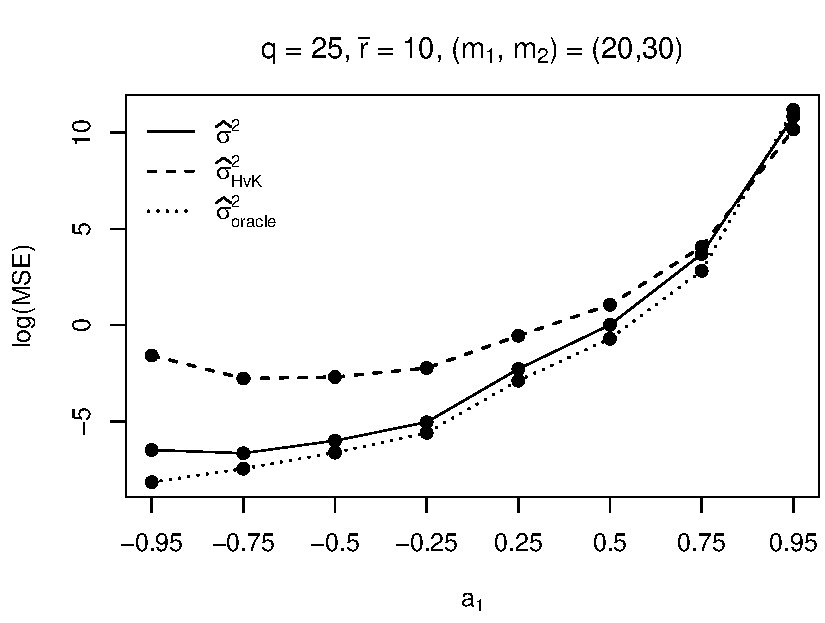
\includegraphics[width=\textwidth]{Plots/Robustness/MSE_lrv_T=500_slope=10_(q,r,M1,M2)=(25,10,20,30).pdf}
\end{subfigure}
\hspace{0.25cm}
\begin{subfigure}[b]{0.45\textwidth}
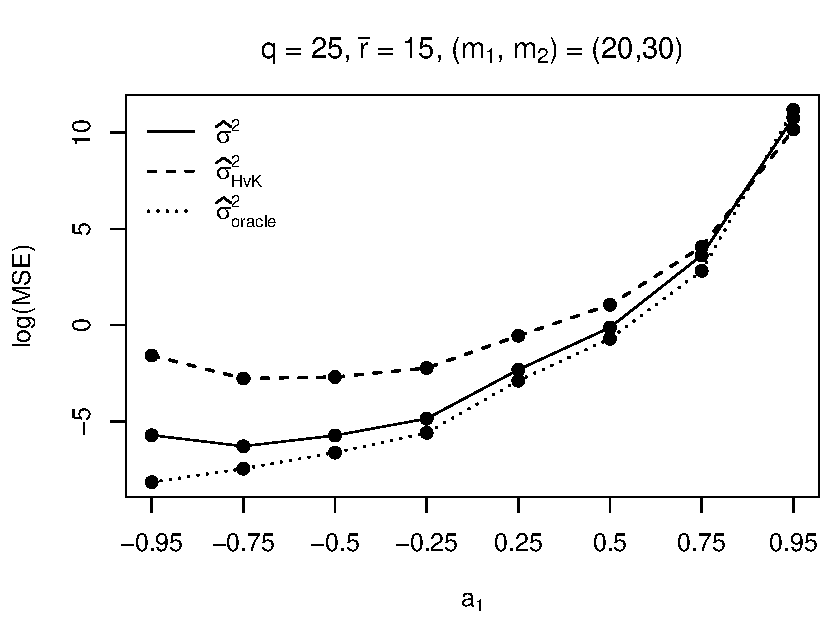
\includegraphics[width=\textwidth]{Plots/Robustness/MSE_lrv_T=500_slope=10_(q,r,M1,M2)=(25,15,20,30).pdf}
\end{subfigure}

\begin{subfigure}[b]{0.45\textwidth}
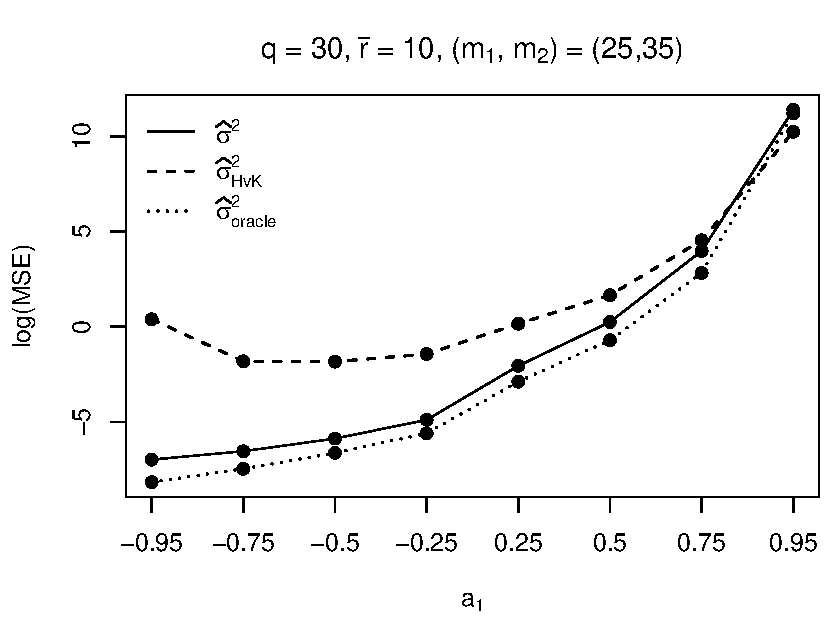
\includegraphics[width=\textwidth]{Plots/Robustness/MSE_lrv_T=500_slope=10_(q,r,M1,M2)=(30,10,25,35).pdf}
\end{subfigure}
\hspace{0.25cm}
\begin{subfigure}[b]{0.45\textwidth}
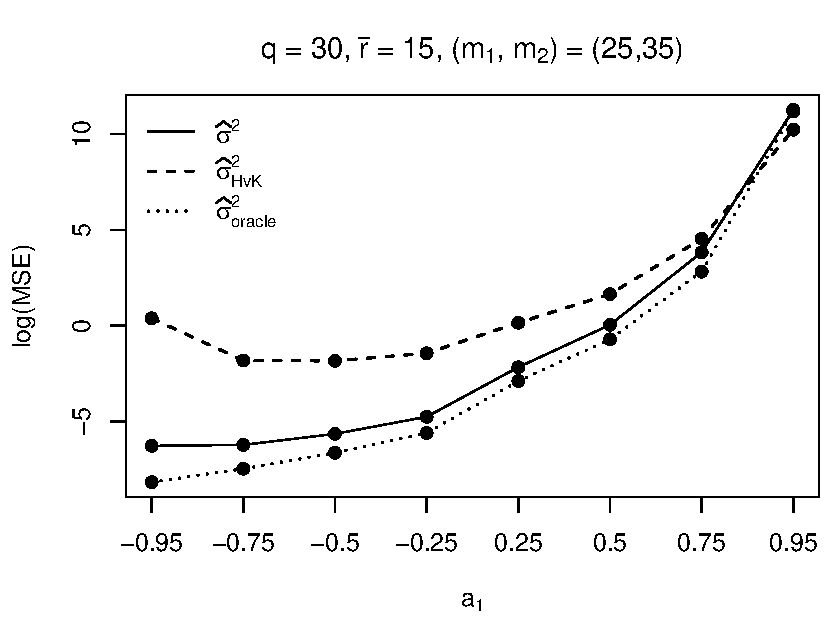
\includegraphics[width=\textwidth]{Plots/Robustness/MSE_lrv_T=500_slope=10_(q,r,M1,M2)=(30,15,25,35).pdf}
\end{subfigure}

\begin{subfigure}[b]{0.45\textwidth}
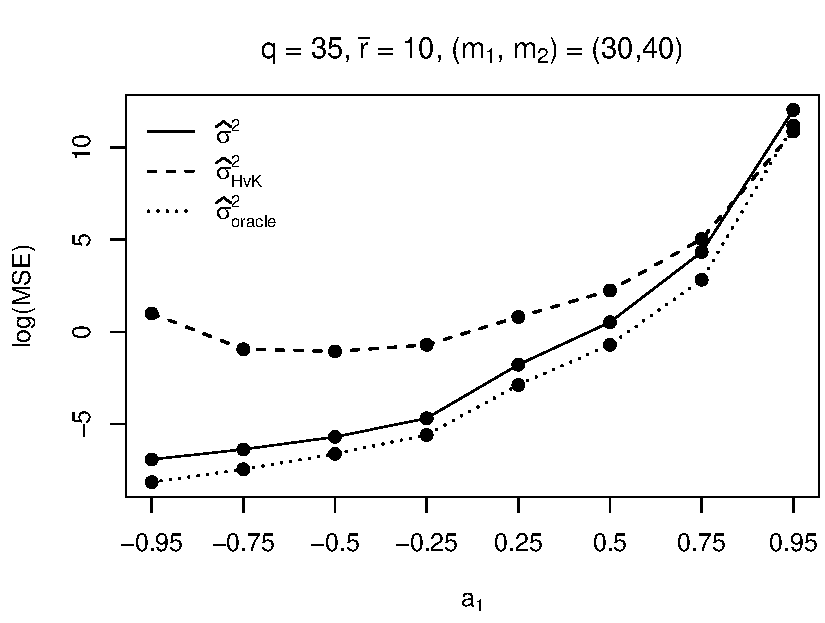
\includegraphics[width=\textwidth]{Plots/Robustness/MSE_lrv_T=500_slope=10_(q,r,M1,M2)=(35,10,30,40).pdf}
\end{subfigure}
\hspace{0.25cm}
\begin{subfigure}[b]{0.45\textwidth}
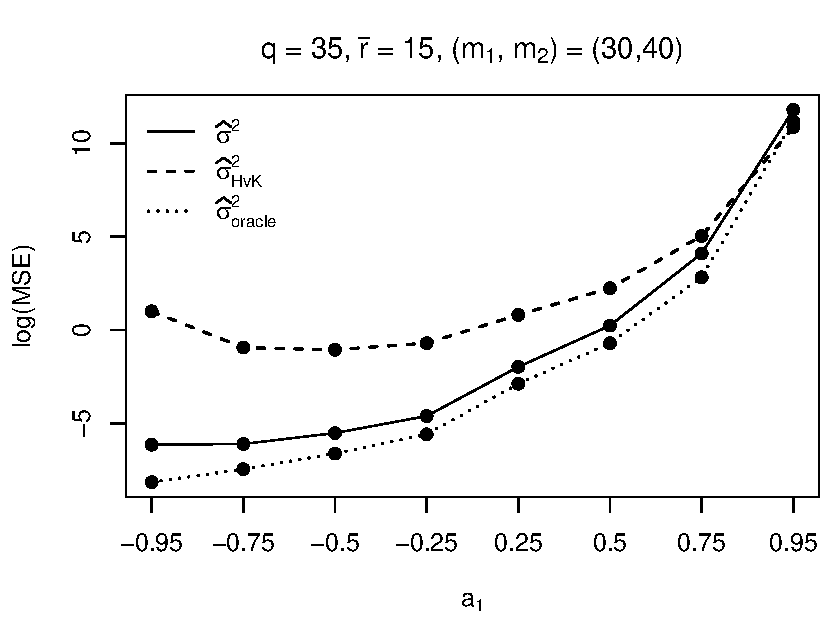
\includegraphics[width=\textwidth]{Plots/Robustness/MSE_lrv_T=500_slope=10_(q,r,M1,M2)=(35,15,30,40).pdf}
\end{subfigure}
\caption{Logarithmic MSE values for the estimators $\widehat{\sigma}^2$, $\widehat{\sigma}^2_{\text{HvK}}$ and $\widehat{\sigma}^2_{\text{oracle}}$ in the scenario with a pronounced trend ($s_\beta=10$).}\label{fig:MSE_slope10_lrv_robust} 
\end{figure}

